\documentclass[12pt, a4paper]{report}
\usepackage[utf8]{inputenc}
\usepackage{times}
\usepackage{caption}
\usepackage{amsmath}% http://ctan.org/pkg/amsmath
\usepackage{array}
\usepackage{pgfplots}
\usepackage[titletoc]{appendix}
\usepackage{graphicx}
\usepackage{subcaption}
\usepackage[a4,frame,center]{crop}
\usepackage[margin=1in,left=1.5in,top=1in, includefoot]{geometry}
\usepackage{chngcntr}
\counterwithout{figure}{chapter}
\counterwithout{equation}{chapter}
%Header and Footer package
\usepackage{fancyhdr}
\pagestyle{plain}
\fancyhead{}
\fancyfoot{}
\renewcommand{\headrulewidth}{1pt}
\renewcommand{\footrulewidth}{0pt}
\lhead{Implementation of Intrusion Detection System in Tensorflow}
\rfoot{Page \thepage}
\usepackage{ragged2e}

\begin{document}

\begin{titlepage}
	\begin{flushleft}
	
\includegraphics[width=14cm]{combine.png}\\
	\end{flushleft}
	\begin{center}
	
	
	\LARGE\bfseries{Otto-Von-Guericke University Magdeburg}\\
	[0.5in ]
	\large {Faculty of Electrical Engineering and Information Technology}\\
	[0.5in]
	\large {Institute for Automation Engineering}\\
	[0.5in]
	\large{Chair for Integrated Automation}\\
	[0.5in]
	\normalsize{\underline {Digital Engineering Project (12 Credits)}}\\
	[0.3in]
	\Huge\bfseries {Implementation of Intrusion Detection System in Tensorflow}\\
	[1in]
	\normalsize {\underline {Supervisor}}\\
	[0.2in]
	Dipl.-Ing. Sasanka Potluri\\
	[0.6in]
	\normalsize {\underline{Project by}}\\
	[0.2in]
	Jay Vala (Matriculation Number - 213739)\\
	Akash Antony (Matriculation Number - 213515)\\
	Kartik Sarin(Matriculation Number - 209893)\\
	\end{center}
	
\end{titlepage}

\pagenumbering{roman}
\tableofcontents 
\thispagestyle{plain}
\listoffigures
\thispagestyle{plain}
\listoftables
\thispagestyle{plain}




\begin{abstract}
\pagenumbering{arabic}
\setcounter{page}{1}
\thispagestyle{plain}
\addcontentsline{toc}{chapter}{Abstract}
\justify
The increasing number of cyber threats in industrial environments has prompted pioneers to search for security solutions that can protect and prevent industries from significant monetary loss and brand erosion. \\ \par
The cyber attacks on Davis-Besse Power Station in January, 2003 and on Iranian Nuclear Plant in December, 2010 has turned industries into finding new and effective ways to tackle cyber security threats in industrial automation. According to Kaspersky lab \emph ``Every month, an average of one industrial computer in five (20.1\%) is attacked by malware.''\cite {Kaspersky}\\ \par
With the rapid adaption and expansion of artificial neural networks for various information and data processing tasks, it is imminent that it will find its use in tackling cyber security. As artificial neural networks are becoming powerful day by day, its power can be harnessed to find the anomalies in industrial network traffic.\\ \par
Stacked Autoencoder and Deep Belief Networks are such artificial neural network which are used for unsupervised learning. A Stacked Autoencoder and Deep Belief Network are multi-layer deep artificial neural networks (DNNs). DNNs are multiple layer architecture which extracts inherent features in data and discover important hidden structure in diverse data sets. This makes them suitable for classification tasks. \\ \par
In this project Stacked Autoencoder and Deep Belief Network were created using Tensorflow, Google's open-source software library for Machine Intelligence.The NSL-KDD dataset was used as it solved some of inherent problems of the KDD'99 dataset. Greedy layer-wise training approach was applied to train our models. Different learning parameters such as different activation functions, different optimizers and variables batch size were also used, there is a command line interface where anyone can tweak these and many more parameters to get optimum results.\\
\end{abstract}

\clearpage
\setcounter{page}{2}
\chapter{Introduction}\label{sec:intro}
\justify
With the exponential increase in computer network usage and the increasing number of devices getting connected to a network, it is of great importance that they are operated securely. All computer networks suffers from one of many security flaws, the recent ``Wannacry Ransomware'' took cyber security industry by storm. Though there was a fix for that security loophole, organizations were slow on applying the security patches, this behaviour of the organization can be because of organizational heirarchial structure, to increase monetory profit or in some cases the machine is operating a critical infrastructure. Therefore, Intrusion Detection System's (IDS) role is becoming important in tackling cyber security.\\ \par

\section{Intrusion Detection System}\label{sec:introintrusion}

\justify
Intrusion detection system can be compared with a burglar alarm \cite{IDS}. For example the alarm system at a house is to protect a house. If somebody who is not authorized to enter the house gets in, it is the burglar alarm that detects and informs the owner of the intrusion in the house or if need be it locks the house. Intrusion detection system in a similar way compliments the firewall security. The firewall protects institution from malicious attacks and it is the job of the Intrusion detection system if someone bypasses the firewall and try to break into or tries to access the system  it alerts the network administrator in case of security breach.\\ \par

However, Firewalls do a great job of filtering out the unwanted incoming traffic into the industrial or institutional network but there may be some cases where external users can connect to the Intranet by dialling in through a modem installed in the private network of the organization.\cite{IDS} This kind of access would not be detected by a firewall.Although Firewalls can be very helpful in repelling intrusions, but they cannot offer any protection against sabotage as the attacker already has trusted access to the company's network and resources. Also hardware firewalls require to be purchased and installed for each network node, which can go very costly.\\
\par

So, an Intrusion Detection Systems (IDS) has more benefits from a firewall as it monitors and analyses the network traffic and checks it for anomalies and abnormalities in the network. If it finds any it creates an alert in the system or informs the system administrator of the attacks whether it is originating from outside and also has the ability to check if the system misuse or attacks are originating from inside the organization.\\ \par

The attacks may be of various types and the system should be able to predict and identify the attacks accurately, without giving false positives, hence the accuracy of the system becomes more important. \\ \par

\section{Classification of Intrusion Detection System}
\subsection{Network Intrusion Detection System}
Network Intrusion Detection System (NIDS) are placed at particularly defined places with in the network to monitor the traffic going in and out of all devices in the network. NIDS are mostly passive devices that monitor the on-going network activity without adding significant overhead or interfering with the network operations. They are easy to install and are secure against attack and may even be undetectable to attackers; they also require little effort to install and use on existing networks. Ideally it would scan all inbound and outbound traffic; however, doing so might create a bottleneck that would impair the overall speed of the network.

\subsection{Host based Intrusion Detection System}
Host based Intrusion Detection System (HIDS) runs on individual hosts or devices on the network. A HIDS monitors the incoming and outgoing packets from the device only and will alert the user or administrator of suspicious activity detected. The suspicious activities are based on the type detection technique employed. For example, audit analyse  technique is able to identify the activities related to operating-system-level intrusion and application-level intrusions.

\section{Advantages of Network Based Intrusion Detection System}\label{sec:advantagesofNIDS}
\begin{enumerate}
	\item {Low Cost of Ownership}
	\item {Easier to deploy}
	\item {Detect network based attacks}
	\item {Retaining evidence}
	\item {Real Time detection and quick response}
	\item {Detection of failed attacks}
\end{enumerate}

\section{Advantages of Host Based Intrusion Detection System} \label{sec:advantagesHostBasedIDS}
\begin{enumerate}
	\item{Verifies success or failure of an attack}
	\item{Monitor System Activities}
	\item{Detects attacks that network based IDS fails to detect}
	\item{Near real time detection and response}
	\item{Does not require additional hardware}
	\item{Low entry cost}
\end{enumerate}


\section{Limitations of Intrusion Detection Systems}\label{sec:limitsofIDS}

Although IDS are very powerful these systems also suffer from many limitations. Noise such as bad packets generated from software bugs, corrupted DNS data can create false alarms \cite{securityengineering}. Outdated expired software versions are generally the target of the attackers, hence a constantly updated signature database has to be maintained in order to tackle these threats \cite{securityengineering}. Also for signature based Intrusion Detection system there is a delay between a new threat detected and the signature being recorded in the database, this can make IDS vulnerable. \\ \par

Taking authentication and identity confirming mechanism into consideration, IDS are helpless against weak authentication when an attacker gains access. A weakness in the network protocol also makes IDS vulnerable. Encrypted packets are not processed by the IDS and this makes it easy for an attacker to send in encrypted packets and gain access to the system. As NIDS analyse the same network protocol as the attacker uses to attack the system, NIDS on its own can become vulnerable and susceptible to such attacks. \cite{limitationOfIDS}
\clearpage



\chapter{Tensorflow}\label{sec:tensorflow}

\section{Introduction}\label{sec:tensor_intro}
\justify
Tensorflow is an interface for expressing machine learning algorithms and an implementation for executing such algorithms. A computation expressed using Tensorflow can be expressed with little or no changes on wide variety of heterogeneous systems \cite{tensorflow_paper}. \\ \par

The Google's Brain project built DistBelief, the first-generation scalable distributed training and inference system. With all the understanding and DistBelief as its core, Google's Brain Team built Tensorflow the second generation of machine learning library. Google and other Alphabet companies have deployed DistBelief and Tensorflow into many of Google's products including Google's search \cite{googleSearch}, Google's Advertising Production, Google's Speech Recognition, Maps, Photos and many more. \\ \par

Tensorflow is highly scaleable and can be mapped on many devices and platform ranging from Android and iOS to large scale system consisting of multi-cpu and multi-gpu configurations. For scaling neural network training to larger deployment, Tensorflow allows parallelism through replication and parallel execution of core model with different computational devices all collaborating to update a set of shared parameters or other states. Modest changes in the description of the computation allows a wide variety of different approaches to parallelism with low effort. Some uses of Tensorflow allows some flexibility in terms of the consistency of parameters updates and we can easily express and take advantage of these relaxed synchronization requirements in some of large deployments.\\ \par

A computation model in Tensorflow is called a \textit{graph}, which in turn composes of set of \textit{nodes}. The graph represents the flow of computation with extension for allowing some kind of nodes to maintain and update its states. Tensorflow supports two front end languages C++ and Python to construct these graphs.\\ \par
\clearpage

\section{Graph Construction and Basic Programming Concept}\label{sec:programmingtensorflow}

As mentioned in section \ref{sec:tensor_intro} a Tensorflow model consists of a \textit{graph} which is composed of \textit{nodes}. These \textit{nodes} has zero or more inputs and zero or more outputs. Values that flow along the edges are called \textit{tensors}. They are nothing but arbitrary dimensional arrays.\\ \par

\subsection{Operations, Kernels, Variables, and Sessions}\label{sec:constituentsoftensorflow}

\subsubsection{Operations and Kernels}\label{sec:ops_kernel}
An operation in its simplest of meaning is calculation of inputs to form output. In Tensorflow, calculation such as ``matrix multiplication'' or ``addition'' are operations. An \textit{operation} in Tensorflow has name and attributes which have to be provided at the time of graph construction. \\ 

A \textit{kernel} is a particular implementation of an operation that can be run on a particular type of devices like CPU or GPU. 


\subsubsection{Variables}\label{variables}
A computation graph is executed many times for a single model, most tensors do not have a persistent state and looses its state after a single execution. Hence, \textit{Variable} which are persistent, mutable handles for storing tensors.


 \subsubsection{Session}\label{session}
A user interact with Tensorflow system by creating a \textit{Session} which creates the computation graph. One primary operation supported by \textit{Session} is \textit{Run} which takes set of output names that needed to be computed, as well as an a set of tensors to be fed to the computational graph and operations are performed accordingly.

\subsection{Tensor}\label{tensor}

A tensor as mentioned above, is an multidimensional array. Tensorflow supports variety of tensor elements including signed and unsigned integers ranging from 8bits to 64bits.

\clearpage

\chapter{Deep Neural Networks}\label{ref:DNN} 

\section{Introduction}\label{sec:intro_dnn}

A Deep Neural Network (DNN) is an Artificial Neural Network (ANN) with multiple hidden layers, input and output layer. Similar to other ANNs, DNNs can model complex non-linear relationships. Because each hidden layers computes a non-linear transformation of previous layer, a DNN can have significantly greater power of representation. DNNs are typically feedforward networks in which data flows from the input layer to the output layer without looping back. However, recurrent neural networks, in which data can flow in any direction, are also used, especially long short-term memory, for applications such as language modeling. Convolutional deep neural networks (CNNs) are used in computer vision. \\ \par

\section{Artificial Neural Network}\label{ANN}
An Artificial Neural Network (ANN) are information processing units that are inspired by the way a human nervous system, such as brain, process information. As human brain processes information and takes decision, these models are designed to do the same. Human brain learns from its day to day experience, these ANN try and replicate the learning process, which makes them suitable for some of the unsolvable and resource hungry task. The key element of these neural networks is a Neuron, this neuron is responsible for all the mathematical operations that are performed such as summation, multiplication etc. When these neurons are highly interconnected in large numbers, they work in unison to solve parts of a bigger problem.\\ \par

ANNs, like human beings learn by examples. An ANN is configured for a specific task or application. These task varies from patten recognition in computer-aided diagnosis, speech recognition to classification of data such as text into various categories. Today ANNs find its use in variety of applications, Google's search are optimized by these neural networks, Facebook's predictive algorithm in news feeds to Amazon's virtual assistant Alexa. \\ \par

Neural Network with their ability to derive meaning from complicated and huge data, that would have been otherwise impossible for either humans or other computer techniques, is what makes it powerful tool. Other advantages include Adaptive Learning, Self Organization, and Fault Tolerance.\\ \par

An artificial neuron is the building block of an ANN. Every input is multiplied with random weights so that the inputs are weighted. These weighted inputs are then summed up with biases and passed through a transfer function and then the net input is passed through the activation function as shown in the Figure \ref{fig:AN}. \\ \par
\begin{figure}[h]
\centering	
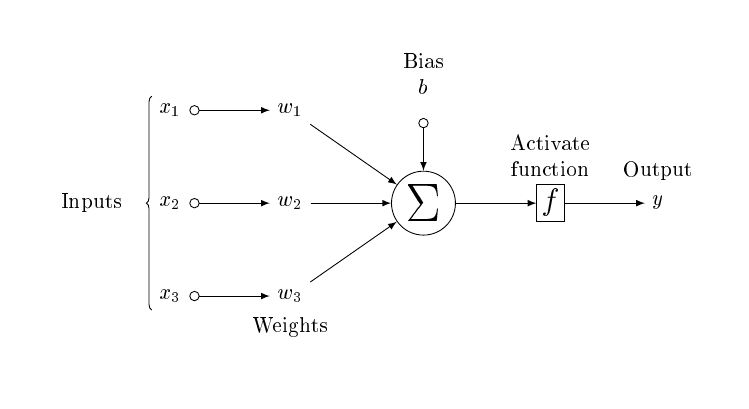
\includegraphics[width=12cm]{ArtificialNeuronModel.png}\\
\caption{Structure of Artificial Neuron}
\label{fig:AN}
\end{figure} 	
\begin{equation}
y=f(x_{1}w_{1}+x_{2}w_{2}+x_{3}w_{3}+b)
\label{Artificial Neuron formula}
\end{equation}\\
\par
Although the structure and computation of a single artificial neuron looks simple and easy, but its full potential and power of calculation is realized when they are interconnected and made into an artificial neural network as show in Figure \ref{fig:NN}\\ \par
\begin{figure}[h]
\centering
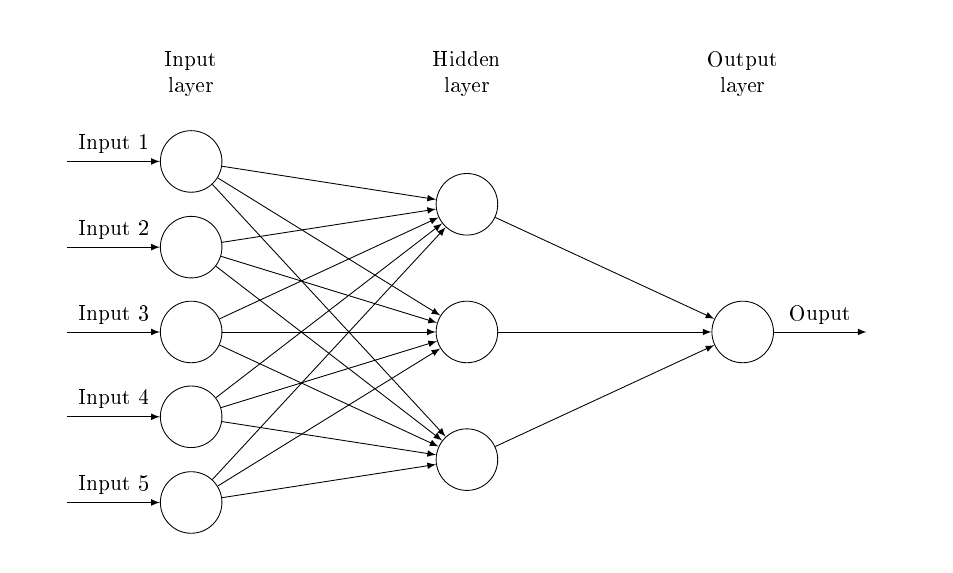
\includegraphics[width=12cm]{neural_network.png}
\caption{Structure of Artificial Neural Network}
\label{fig:NN}
\end{figure}

These artificial neural networks are interconnections of artificial neurons, however these neurons can not be connected in any way. There are predefined architectures and topologies which make them more beneficial to use. These architectures are very effective in numerous tasks and can solve problems quickly and effectively. Once we know the type of problem we need to solve, then we can select appropriate  architecture or topology for the artificial neural network and run our model.\\ \par

Once the appropriate topology is selected, then we are ready to train our model. Just like a human brain which learns its responses from the inputs  from all the sensory organs, for an artificial neural network to do whatever its intended to do it requires training. There are two phases of training, one is pre-training and another is fine tuning phase. As ANN is successful in solving the problems we have provided, then it can be used for solving the problem we intended. Artificial neural networks are used in the fields of chemistry, medicine, banking, stock market. It can also solve problems like facial recognition, time-series prediction, regression analysis, pattern recognition.


\section{Artificial Neural Networks: Types}

As we know the building block of Artificial Neural Network (ANN) is the artificial neuron, and when we have more then two artificial neurons working together, we have an artificial neural network. A single neuron is not powerful enough to solve big complex real world problems, but when they are put together in a specified topology or architecture they can be very handy in solving the same task a single neuron fails to perform. Advantage of artificial neural network is that these neurons can process data in distributed way, in parallelly, non-linearly and locally. \\\par

The ways in which these neurons are connected is what makes them so powerful. There are basically two main topologies in which these neurons are connected. 
\begin{figure}[h]
\centering
  \begin{subfigure}[b]{0.4\textwidth}
    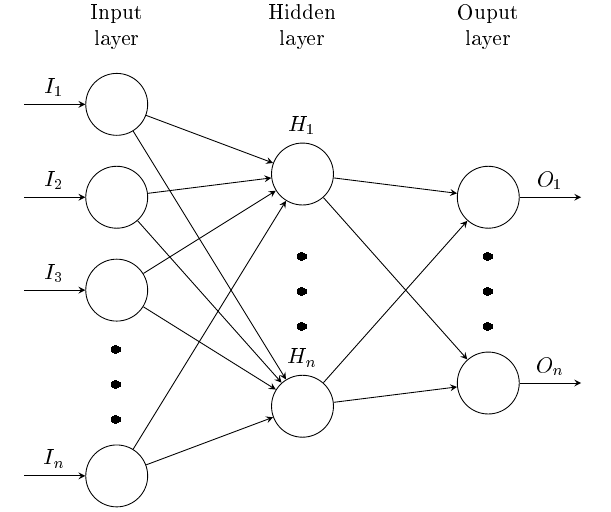
\includegraphics[width=\textwidth,height=4cm]{nn_2.png}
    
  \end{subfigure}
  %
  \begin{subfigure}[b]{0.4\textwidth}
    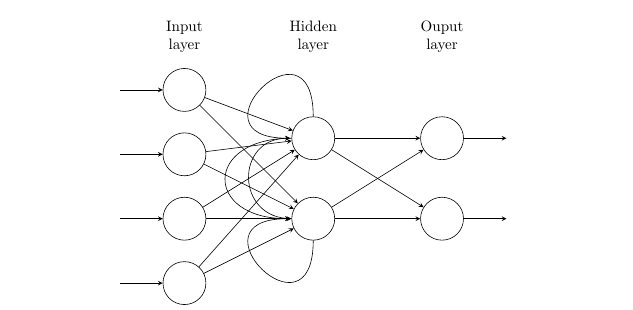
\includegraphics[width=9cm,height=4cm]{rnn.png}
  \end{subfigure}
  \caption{Feed Forward and Recurrent Neural Network}
 \label{fig:FFRN}
\end{figure}

As we can see from the Figure \ref{fig:FFRN} that in feed forward neural network the flow of information is only in one direction that is from inputs to the outputs wherein in the recurrent neural network the information flows in many possible directions as show in the Figure \ref{fig:FFRN} \\ \par

There are other neural networks as follows
\begin{itemize}
	\item Convolutional Neural Networks
	\item Long sort-term memory
	\item Deep Belief Networks
	\item Stacked Auto-encoders
	\item Hopfield Neural Networks 
	\item Elman and Jordan Artificial Neural Networks
	\item Generative Adversarial Networks
	\item Boltzmann and Restricted Boltzmann Machines
\end{itemize}
\section{Training a Deep Neural Network}\label{train}

Training a neural network \textit{Deep or Shallow} requires some parameters to be set. These parameters are important in a way that is it determines the way a neural network will be producing results. Once the structure of the network is decided that is how many layers would be needed for that specific task and what will be the number of neurons in each layer, will you be needing a shallow or a deep network. After the structure of the neural network is decided upon then it has to be decide what \textit{activation function} is to be used, what will be the learning algorithm to be used, how many epochs will be needed, what kind of learning will be needed, will it be supervised, unsupervised or reinforcement learning. These parameters will decide what kind of output will it be producing.\\ \par

\subsection{Supervised Learning}\label{sec:supervisedLearning}

Supervised Learning is similar to how a human brain learns. Inputs and corresponding outputs are given to the network, this makes it easy for the network to classify or recognize the inputs as they are, then a new set of inputs are given to the network which the network has never seen before and its told to recognize based on the previous learning. Initially the weights are randomly selected and the neural network then maps the inputs and compares the corresponding outputs to the given labels or targets. Based on the comparison an error signal is generated, ideally the error signal is zero if the outputs are equal or similar to the inputs given, this error signal is then back propagated to the network. System then adapts its weights according to the error signal and optimize the error to make it more accurate. The repetitive process minimizes the error signal to a point where it is within our error tolerance level. Figure \ref{fig:supervised} shows how the error calculated at the end is back propagated to the network.\\ \par

Some of the supervised learning algorithms are listed below
\begin{itemize}
	\item{Perceptron Learning}
	\item{Back-propagation}
	\item{Newton Method}
	\item{Grossberg Learning}
\end{itemize}

\begin{figure}[h]
\centering	
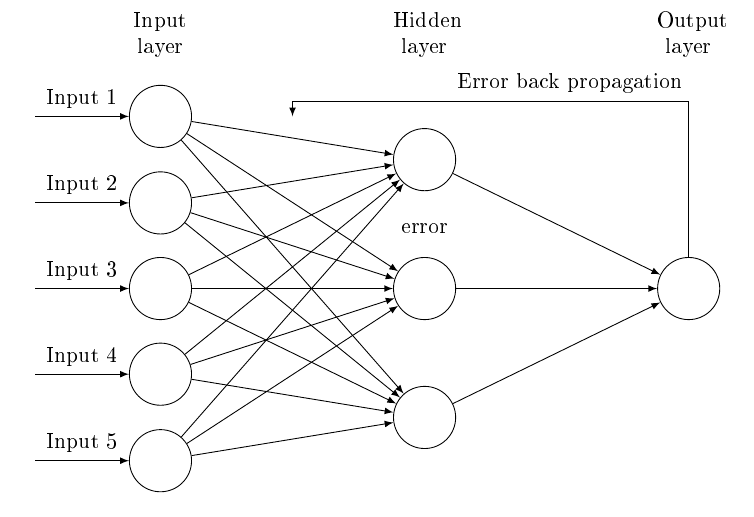
\includegraphics[width=9cm]{supervised.png}\\
\caption{Supervised Learning}
\label{fig:supervised}
\end{figure} 


\subsection{Unsupervised Learning}\label{sec:unsupervised}

Contrary to supervised learning, in unsupervised learning only inputs are provided and no outputs is provided. Input data is then grouped together and the network is trained on the features decided by the model itself. It learns the hidden structure and representation of the data. 
Many approaches uses unsupervised learning, some of them include clustering, where dataset given is to be clustered or grouped together based on their similarities. In artificial neural networks Generative adversarial networks (GAN) uses unsupervised learning, implemented by a system of two neural networks competing against each other in a zero-sum game framework\cite{unsupervised}.\\ \par
An example of unsupervised learning is clustering, in the Figure \ref{fig:cluster} \textit{k-means} clustering is seen where \textit{k=2}, hence the data is clustered into two different clusters based on their structure.\\ \par
Unsupervised learning approaches include

\begin{itemize}
	\item{Clustering}
	\item{Generative Adversarial Networks(GAN)}
	\item{Hebbian Learning}
\end{itemize}
\par
\begin{figure}[h]
\centering	
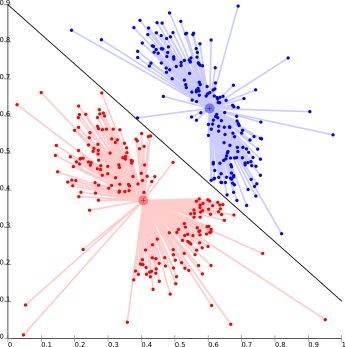
\includegraphics[width=7cm]{cluster.png}\\
\caption{Unsupervised Learning(K-Means)}
\label{fig:cluster}
\end{figure} 

\subsection{Reinforcement Learning}\label{sec:ReinforcementLearning}

Reinforcement learning is inspired by behaviorist psychology. As the name suggest it reinforces itself to maximize the performance of the network. Reinforcement learning is different from other learning in a sense that in reinforcement learning we do not provide pair of input and output data, rather an agent takes an action in an environment which is then interpreted by an interpreter or critic which then rewards the agent accordingly and this feedback is then analyzed and agent improves its performance in accordance to the reward.\\ \par

\begin{figure}[h]
\centering	
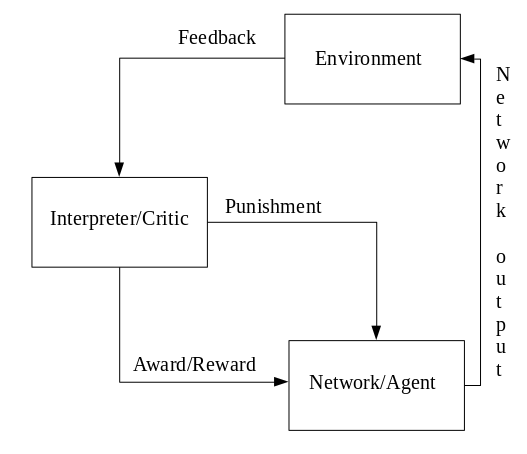
\includegraphics[width=6.9cm]{reinforcement.png}\\
\caption{Reinforcement Learning}
\label{fig:reinforcement}
\end{figure} 

\clearpage

\subsection{Activation Functions}\label{activationfunction}
Activation function in a neural network can be described as a function which transfers or translates the input signal to output signal. Comparing it to electrical circuit an activation function is one which can be ``\textit{ON}'' (1) or ``\textit{OFF}'' (0) depending on the input it receives. As the artificial neurons are inspired by the biological neuron, the activation function in biological from is either the neuron is firing or not.\\ \par

Activation functions are selected for a specific application and are highly application dependent. There are many applications which needs classification and there are many application which require prediction, hence the properties of different activation's are used in different applications. The most common activation functions with its properties are listed below. However we have used only four of the activation functions namely \textit{Sigmoid Activation, ReLU activation, eLU activation, Softplus activation} and in all the models the last layer of the model has \textit{Softmax activation}.\\ \par

\subsubsection{Sigmoid Activation Function}\label{sec:sigmoid}
Sigmoid is one of the most common activation function used in neural networks. This function is widely used because its easy to calculate their derivatives, which makes weights calculation very easy in some cases. Sigmoid activation has the vanishing gradient problem.\\ \par
%equation of sigmoid
\begin{equation}
S(x) = \frac{1}{1-e^{x}} \\
\label{eq:sig}
\end{equation}

%graph of sigmoid
\begin{figure}[h]
\centering	
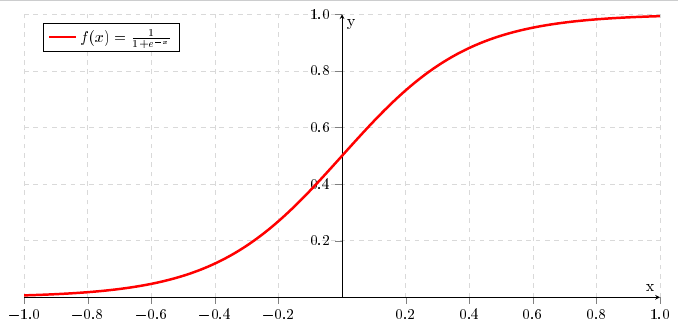
\includegraphics[width=12cm]{sigmoid.png}\\
\caption{Sigmoid Activation Function}
\label{fig:sigmoid}
\end{figure} 	
\clearpage
\subsubsection{Step Function}\label{sec:step}
Step function was used in perception. The output is certain value, if the sum of the inputs is above or below a certain threshold. These kind of activation functions were used in case of binary classification. In other words, if there are only two classes to classify we can use this activation function.\\ \par
%equation of step
 \begin{equation}\label{eq:step}
f(x) = \begin{Bmatrix}
1 & x \in A \\ 
0 & x \notin A 
\end{Bmatrix}
\end{equation}

%graph of step
\begin{figure}[h]
\centering	
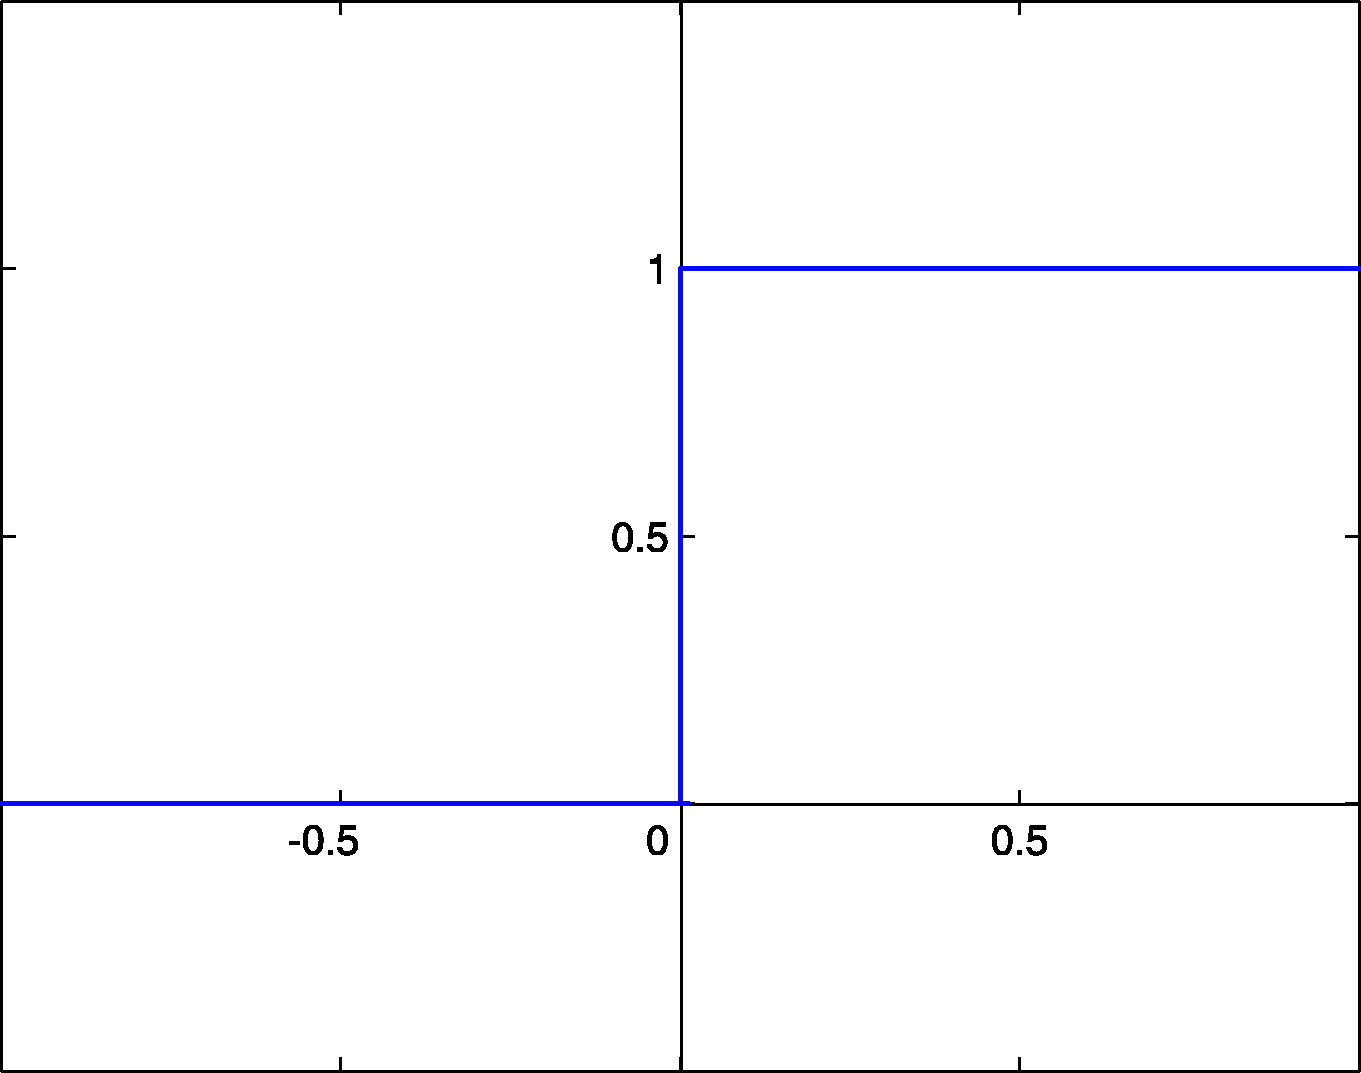
\includegraphics[width=5cm]{step.png}\\
\caption{Step Activation Function}
\label{fig:step}
\end{figure} 	

\subsubsection{Rectified Linear Unit (ReLU)}\label{sec:ReLU}
Rectified Linear Unit function was first introduced by Hahnloser in 2000  with strong biological motivation and justification. This is the most popular activation function from deep neural networks,because unlike Sigmoid and TanH activation ReLU does not have a vanishing gradient problem\cite{ReLU}.\\
%equation of relu
\begin{equation}\label{eq:ReLU}
f(x) = \begin{Bmatrix}
0 & x < 0 \\ 
x & x \geq 0 
\end{Bmatrix}
\end{equation}
%graph of relu
\begin{figure}[h]
\centering
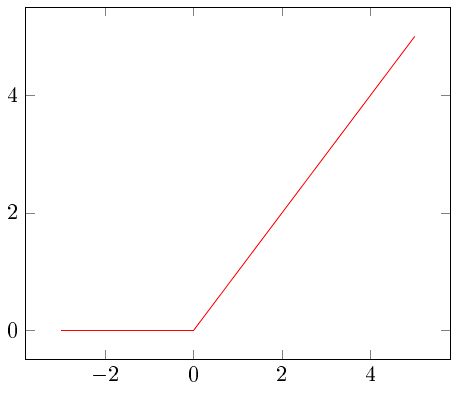
\includegraphics[width=6.5cm]{relu.png}
\caption{Rectified Linear Unit Activation Function}
\label{fig:ReLU}
\end{figure} 

\subsubsection{TanH Activation Function}\label{sec:tanh}
TanH activation function has characteristics similar to sigmoid activation function, its a scaled sigmoid. It is nonlinear in nature, and its gradient is stronger than sigmoid. Deciding on which to use will depend on the application. Like sigmoid, TanH also has the vanishing gradient problem.
%eq 
\begin{equation}\label{eq:tanh}
f(x) = tanh(x)=\frac{2}{1+e^{-2x}} -1
\end{equation}
%fig
\begin{figure}[h]
\centering
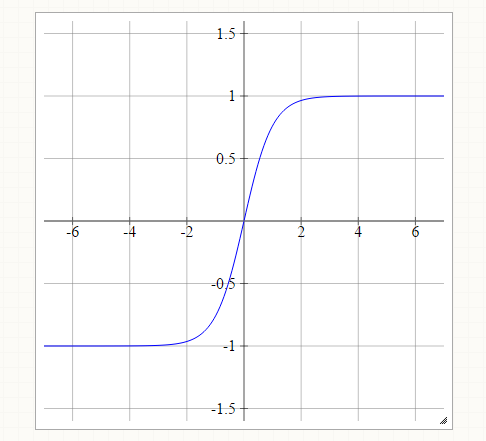
\includegraphics[width=6.5cm]{tanh.png}
\caption{TanH Activation Function}
\label{fig:tanh}
\end{figure} 

\subsubsection{Exponential Linear Unit (eLU)}\label{sec:ELU}
Exponential Linear Unit alleviate the vanishing gradient problem via the identity for positive values. However, Exponential Linear Units have improved learning characteristics compared to the units with other activation functions \cite{ELU}.\\ \par
%formula
\begin{equation}\label{eq:ELU}
f(\alpha ,x) = \begin{Bmatrix}
\alpha(e^{x}-1) & x<0\\ 
x & x\geq 0 
\end{Bmatrix}
\end{equation}

\subsubsection{Softmax Activation Function}\label{sec:softmax}
Softmax activation function is a generalization of the logistic function, in probability theory the output of the softmax function can be used to represent a categorical distribution, that is a probability distribution over \textit{X} possible outcomes. Hence, softmax activation function is used in various multi-class classification in artificial neural networks.\\ \par
%equation forsoftmax
\begin{equation}\label{eq:softmax}
f_{i} (\overrightarrow{x}) =\frac{e^{x_{i}}}{\sum_{j=1}^{J} e^{x_{i}} }     \forall \textit{i=1...J}
\end{equation}
\\ \par

\subsubsection{Softplus Activation Function}\label{sec:softplus}
Softplus activation function is considered to be "smooth version of ReLU". Softplus has nonzero derivative everywhere on the graph which is contrast to ReLU.


\begin{equation}\label{eq:softplus}
	f(x) = ln(1+e^{x})
\end{equation}
\begin{figure}[h]
	\centering
	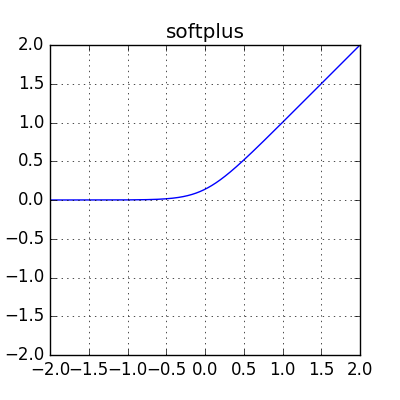
\includegraphics[width=7cm]{activation-softplus.png}
	\caption{Softplus Activation Function}
	\label{fig:softplus}
\end{figure}


%optimizers k formulas Likhna hai..

\subsection{Optimization Algorithm}\label{optimizer}

Optimization algorithms in neural networks helps in minimizing or maximize a loss function which is simply a mathematical function dependent on models internal parameter which calculates models inability in computing the target values from the set of predictions. The internal parameters such as weights and biases values of a neural network which plays a major role in training process of the neural network, optimizing algorithm helps in setting the values such that there is practically no difference between the predicted value and the value that was feed to the network.\\ \par

In this project of ours we have used four different optimizers to minimize the loss function, namely \textit{Adam Optimizer, Stochastic Gradient Descent optimizer, RMSProp Optimizer, Momentum Optimizer}

\subsubsection{Stochastic Gradient Descent Optimizer}\label{sgd}
Gradient descent is also called steepest descent. It is used to find the minimum of a function. It is also the popular method in the field of machine learning to find the highest accuracy and to minimize the error rate of a given training set and is used to calculate the minimum error by minimizing the cost function . To find the gradient descent, we need to take some steps which are proportional to the negative of the gradient of the function at a point. And if we take steps which are proportional to the positive gradient it reaches the local maximum of that particular function. This is known as gradient ascent\cite{OptimizerGeneral}.\\ \par

\begin{gather}\label{eq:autoencoder_eq}
w = w- \eta\sum_{i=1}^{n} \nabla Q_{i}(w)/n
\intertext{Where:}
  \begin{tabular}{>{$}r<{$}@{\ :\ }l}
    w & is the parameter to be estimated\\
    Q_{i}(w) & is is the value of the loss function at the i-th example\\
    \eta & is the step size (sometimes called the learning rate in machine learning)\\
  \end{tabular}\nonumber
\end{gather}
\\ \par

\subsubsection{Adam Optimizer}\label{adam}
ADAM (Adaptive Moment Optimizer) is an extension to GradientDescent optimizer which is seen these days as a broader option for deep learning applications in case of computer vision and natural language processing. It is used instead of GD to update the weights in the network based on iterations in the training data and is used to calculate the adaptive learning rate for each parameters (weight and bias)\cite{OptimizerGeneral}. It’s an popular algorithm in deep learning and have shown good results combining the properties of both AdaGrad and RMSProp algorithms which could handle the noise problems\\ \par

\subsubsection{Momentum Optimizer}\label{momentum}
It is used to accelerate the learning using SGD. If gradient descent is navigating down a valley with steep sides, it tends to madly oscillate from one valley wall to the other without making much progress down the valley. This is because the largest gradients point up and down the valley walls whereas the gradient along the floor of the valley is quite small. Momentum Optimization attempts to remedy this by keeping track of the prior gradients and if they keep changing direction then damp them, and if the gradients stay in the same direction then reward them. This way the valley wall gradients get reduced and the valley floor gradient enhanced.\cite{momentum}\\ \par

\subsubsection{RMSProp Optimizer}\label{RMSProp}
It is able to increase or decrease the learning rate which the other optimizer named Addgradis not able to. In RMSProp overall learning rate will be divided by the square root of the sum of squares of the previous update gradients for a given parameter. The difference is that RMSProp doesn’t weight all of the previous update gradients equally, it uses an exponentially weighted moving average of the previous update gradients which means that the old error values doesn’t contribute much \cite{OptimizerGeneral}. In this way this optimizer jumps around the optimum.



\section{Challenges in Training a Deep Neural Network}\label{challenges}

Deep Neural Networks are comprised of multiple hidden layers, so many issues can arise while training a DNN. Three most common issues are \textit{Overfitting}, \textit{Computation time} \textit{Underfitting.}\\ \par

DNNs are prone to overfitting because of the added layers of abstraction, which allows them to model rare dependencies in the training data. Regularization methods such as weigh decay (l2- regularization) or sparsity (l1 regularization) can be applied during the training of the model to combat overfitting\cite{challenge1}.\\\par

Training a DNN with multiple hidden layers consisting of hundreds of thousands of neurons can be a lengthy and time consuming process. Considering many training parameters such as size, the learning rate, initial weights,biases and trying each and every possible combination can be a time consuming process and may not even be a feasible process\cite{challenge2}. Various methods such as batch size, parallel processing and distributed computing can speed up the computation process. Use of GPU's can also speed up the process.\\ \par

\section{Stacked Autoencoder}\label{Autoencoder}
An autoencoder is an simple artificial neural network first introduced in 1980 by Hilton and the PDP group \cite{autoencoder}. Autoencoders are used for unsupervised learning. They were introduced to address the problem of ``backpropagation without teacher'', by using inputs as teacher \cite{autoencoder2}. The aim of an autoencoder is to learn a representation of a data. Recently, the autoencoders have become widely popular and used for learning generative models in unsupervised pre-training.\\ 
\par

\subsection{Structure}\label{structure}

In its simplest form an autoencoder is a feedforward, non recurrent model. It can be generalized as a network having input layer, output layer and hidden layer. A stacked autoencoder is nothing but a network we get by stacking hidden layers onto one another and making it a deep architecture. The output layer has same number of nodes as the input layer with the purpose of reconstruction of the inputs. In our case we had to classify the attacks in a network into five classes hence there will be five neurons in the output layer.\\ \par

In simplest of the cases, where there is only one hidden layer the mathematical representation of autoencoder will be,

\begin{gather}\label{eq:autoencoder_eq}
y = \sum_{i=0}^{n} \sigma(W_{i}x_{i} +b_{i})
\intertext{Where:}
  \begin{tabular}{>{$}r<{$}@{\ :\ }l}
    y & is the output of the network\\
    i & is the number of neurons in a layer\\
    \sigma & is the activation or the transfer function\\
   W& is the weights vector   \\
    x & is the values of input signal \\
    b & is the values of bias added \\
  \end{tabular}\nonumber
\end{gather}
\\ \par
\begin{figure}[h]
\centering
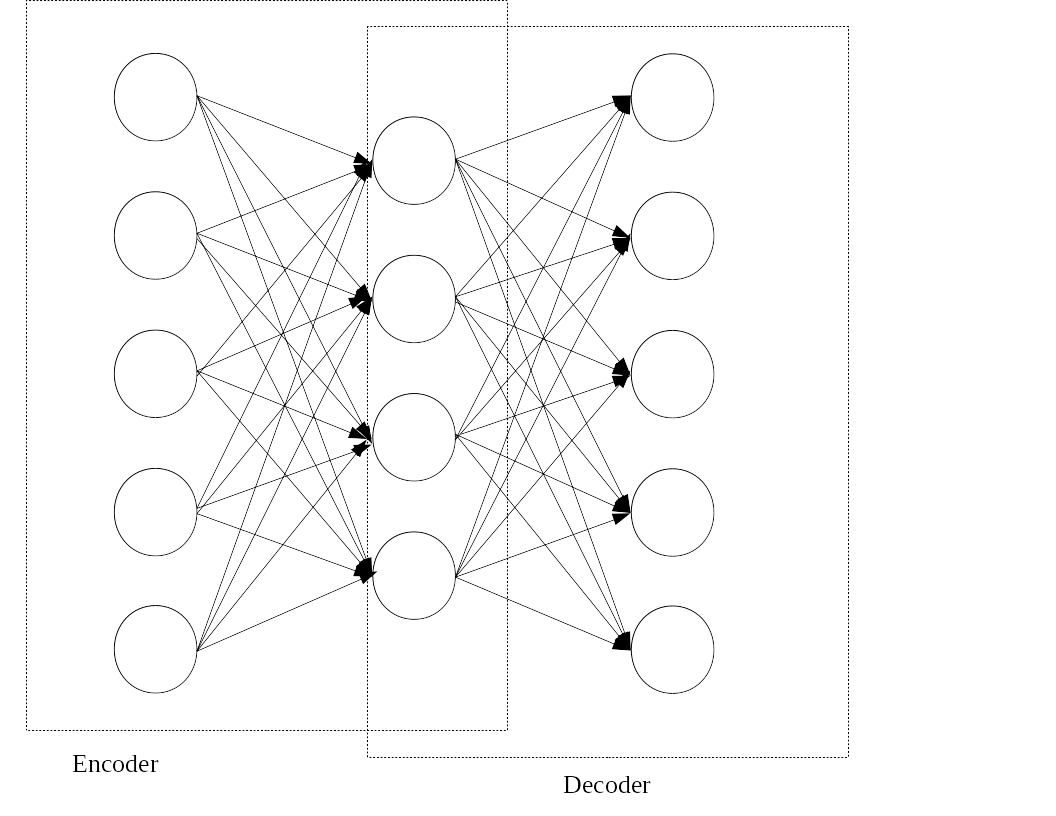
\includegraphics[width=8cm]{autoencoder.png}
\caption{Autoencoder with single hidden layer}
\label{fig:autoencoder}
\end{figure}


\subsection{Types of Autoencoders}\label{sec:types_autoencoder}

The simple autoencoder have some disadvantages, in some cases it was unable to learn the important features effectively. Hence, there was a need for improving the ability of autoencoders to learn the important features and representations for highly accurate results, and hence there was need of Denoising and Sparse autoencoders .\\ \par

\subsubsection{Denoising Autoencoders}\label{sec:denoising_autoencoder}

When an autoencoder is trained, its necessary that the inputs provided for training purpose are not corrupted. After the training is done and the model is applied to a real world problem there is a possibility that the inputs given to autoencoder are corrupted, this may destabilize the model, and the results may not be robust. In order to tackle this problem, in \textit{Denoising autoencoder} takes partially corrupted inputs in the training phase to recover the uncorrupted inputs.\\ \par

\subsubsection{Sparse Autoencoder}\label{sec:sparse_autoencoder}

In \textit{Sparse autoencoder}, we have large number of hidden units, more than inputs, by doing so the autoencoder can learn more useful structures and representation of the data. This kind of autoencoder is useful in classification tasks. Also sparsity can be achieved by tweaking the loss function during training (comparing probability distribution of the hidden unit activation with some low desired values) or by manually choosing the strongest hidden activation functions and ignoring the rest refereed to as \textit{k-sparse autoencoders}\cite{ksparseautoencoder}.\\ \par

The difference between Stacked autoencoder, Denoising autoencoder and Sparse autoencoder is that when we stack number of layers of encoder and similarly the decoders what we get is Stacked Autoencoders. This stacking helps in learning robustly the underlying structure in the data, Denoising Autoencoders are different in a way that it takes inputs with noise which makes it robust for any real world data and less susceptible to instability. Sparse autoencoders like stacked autoencoder also helps in understanding the underlying structure of the input data.

\section{Deep Belief Networks}\label{sec:deep_belief_network}

Deep Belief Networks are probabilistic generative models that are composed of multiple layers of stochastic, latent variables. The latent variables are binary units and are often called feature detectors\cite{DBN}. There is connection between units of different layers but not within the layers.
A deep belief network is stacked \textit{Restricted Boltzmann Machines} (RBM), in which each RBM layer communicates with previous and subsequent layer, but the nodes of any single layer don't communicate with each other.

\subsection{Restricted Boltzmann Machine}\label{sec:RBM}

A \textit{restricted boltzmann machine}(RBM) is a generative stochastic artificial neural network that can learn a probability distribution over a set of inputs. RBMs were invented by Harmonium by Paul Smolensky in 1986\cite{RBM}. RBMs have found their uses in dimentionality reduction, classification, collaborative fitting, feature learning and topic modelling\cite{RBMuses}. They are variant of Boltzmann Machines, with the restrictions that their neurons must form a bipartite graph, and nodes in same layer have no connection between themselves. In Figure \ref{fig:RBM}, \textit{h} is the hidden units and \textit{x} is the inputs.\\ \par

\begin{figure}[h]
\centering
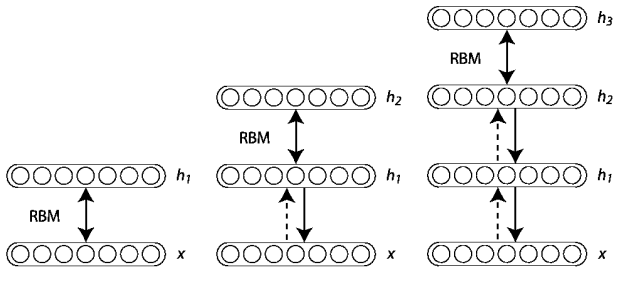
\includegraphics[width=9.5cm]{DBN.png}
\caption{Deep Belief Network}
\label{fig:RBM}
\end{figure}

\subsection{Greedy Layer-Wise Training of Neural Networks}\label{greedy}
As we have seen already seen in section \ref{challenges} that training a deep architecture of neural network is challenging. So the question remains how can we train deep networks? Geoffrey Hilton proposed greedy layer-wise training algorithm to train Deep Belief Networks \cite{Greedy}. The process involves is to train the layers of a network one at a time, suppose we have a deep neural network of four layers, so first we train a network with one hidden layer and after the first layer is trained we save the weights and biases. After the training is done we add a new layer and train again, in the end we save all the weights and biases, then we train the whole neural network with the weight and biases initialized from the saved ones from pre-training of each layer.\\ \par


\chapter{Evaluation and Results}\label{sec:EvaluationAndResults}
\section{The Approach}\label{approach}

\subsection{Parameters}
\subsubsection{Learning Rate}
\textit{Learning rate} is a training parameter that decides how quickly the weight and biases of the neural network are updated during the learning process. This factor is as important as other because if the learning rate is too high then the problem of \textit{overfitting} arises and if the learning rate is too low then it would not reach the local minima for the decided number of iterations. There is no definitive way to know what learning rate should be used, but to do multiple iterations and get the idea of what the learning rate should be.\\

\subsubsection{Epochs}
One \textit{Epoch} is the one forward and one backward pass of \textbf{all} the training samples in a neural network. Suppose we have 10,000 training samples, than one epoch will be feed pass of all the 10,000 training samples and then one backward pass of the same 10,000 training samples, although these samples will be divided into batches.\\

\subsubsection{Batch Size}
It is the number of training examples in one forward and backward pass. Here test set in NSL-KDD dataset has 22,542 records with 41 features, the representation of which is [22542,41], the batch size we has is \textit{10} so this means it will take [10,41] matrix and feed it to the neural network for forward and backward pass 2254 times in one epoch.\\

The following attributes were evaluated for all both the models.\\

\subsubsection{Accuracy}
Accuracy is the percentage measure of correctly classified or identified records over the total number of records.\\

\subsubsection{Precision (P)}
Referred as Positive Predictive Value (PPV)  defined as the percentage ratio of the number of \textit{True Positive (TP)} records divided by the sum of \textit{True Positive} and \textit{False Positive (FP)} classified records.\\ \par
\begin{equation}
Precision = \frac{TP}{TP+FP}
\end{equation}

\subsubsection{Recall (R)}

Referred as the TP rate as sensitivity defined as the percentage ratio of number of \textit{True Positive (TP)} records divided by the sum of \textit{True Positive (TP)} and \textit{False Negative (FN)} classified records

\begin{equation}
Recall = \frac{TP}{TP+FN}
\end{equation}

\subsubsection{F-Measure (F1-Score)}
A measure to represent test accuracy defined as the harmonic mean of precision and recall and represents a balance between them.
\begin{equation}
F-Measure =	2*\frac{P*R}{(P+R)}
\end{equation}

Testing and evaluating the model is performed with some fixed settings. The number of epochs taken are \textit{80}, the learning rate of \textit{0.001} and batch size of \textit{10}. 
\clearpage
\section {Data Set Evaluation}\label{sec:datasetEvaluation}

There are 3 datasets available to us in NSL-KDD dataset. A generalized neural network need \textit{train data} for training a neural network, \textit{test data} to evaluate the model with different parameters and a \textit{validation set} to validate the training of a model. Here we have all three dataset with their labels as well.\\ \par

However, the distribution of the attack types in each are different. In test data set there are total of 22,542 records and in train data set there are 1,25,972 records.  
The distribution of attack types in both test and train set is shown in \ref{table:test_train}\\ \par 
\begin{table}[h]
\centering
\begin{tabular}{|c|c|c|}
\hline
\textbf{Attack Types} & \textbf{Number of records in Train Set} & \textbf{Number of records in Test Set} \\ \hline
Normal                & 67342                                   & 10003                                  \\ \hline
DoS                   & 45927                                   & 7164                                   \\ \hline
Probe                 & 11656                                   & 2421                                   \\ \hline
U2R                   & 995                                     & 2887                                   \\ \hline
R2L                   & 52                                      & 67                                     \\ \hline
\end{tabular}
\caption{Distribution of records in Test and Train Set}
\label{table:test_train}
\end{table}

The dataset used for traning is \textit{Test Dataset} and the dataset used for testing is \textit{Train Dataset.}

\section{Stacked Autoencoder}\label{sec:autoencoder}

\subsection{Results}\label{results}

Implementation of stacked autoencoders was done in different ways and two libraries. Doing so will give us a better view on which parameters work well for what configurations. In the following sections, the evaluation of stacked autoencoder in Greedy Layer-Wise pre-training can be found. The evaluation of stacked autoencoder in non greedy training with TFlearn library can be found in appendix \ref{app:super} and results of stacked autoencoder in non greedy training in Tensorflow can be found in appendix \ref{app:unsuper_tf}.

\clearpage
The settings used to evaluate this model are depicted below, if due to some reason the settings are tweaked then it will be mentioned beforehand.\\ 

\begin{table}[ht]
\centering
\begin{tabular}{|c|c|}
\hline
\textbf{Parameters} & \textbf{Values} \\ \hline
Learning Rate       & 0.1             \\ \hline
Pre-Training Epochs & 10              \\ \hline
Fine Tuning Epochs  & 10              \\ \hline
Batch Size          & 100             \\ \hline
\end{tabular}
\caption{Configuration of Autoencoder for Greedy Layer-Wise Pre-Training}
\label{config_auto_greedy}
\end{table}

\subsection {Adam Optimizer}
\begin{figure}[ht]
\centering
\captionsetup{justification=centering,margin=2cm}
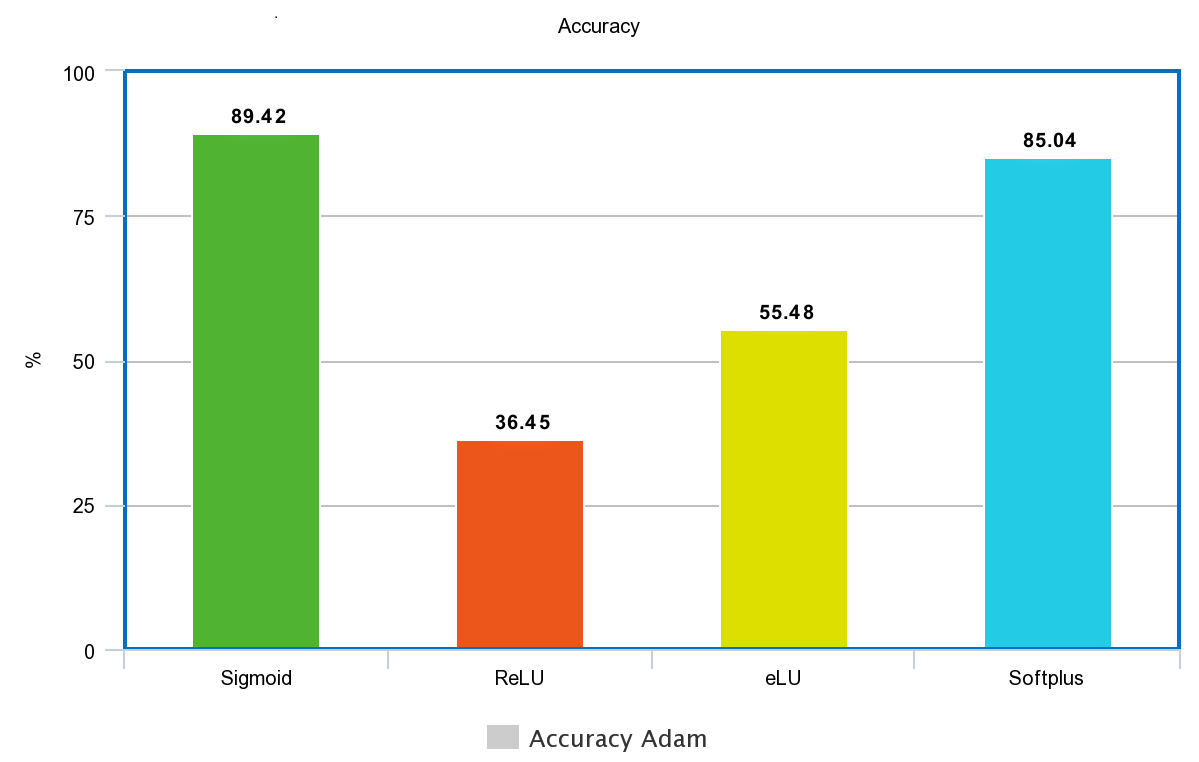
\includegraphics[width=13cm]{adam_accuracy_greedy.png}
\caption{ Accuracy of Adam Optimizer for different activation functions}
\label{fig:accuracy_adam_greedy}
\end{figure}

Figure \ref{fig:accuracy_adam_greedy} shows that sigmoid and softplus activation functions have good accuracy compared to ReLU and eLU activation functions.
We have also analysed all the attack types correctly predicted by different activation functions as show in table \ref{confusion_adam}
\clearpage
\begin{table}[ht]
\centering
\captionsetup{justification=centering,margin=2cm}
\begin{tabular}{|c|c|c|c|c|c|}
\hline
\textbf{Attack Types} & \textbf{Total Samples} & \textbf{Sigmoid} & \textbf{ReLu} & \textbf{eLu} & \textbf{Softplus} \\ \hline
\textbf{Normal}       & 67342                  & 61293            & 0         & 64074        & 67000             \\ \hline
\textbf{DoS}          & 45927                  & 43761          		  & 45927         & 0         & 40137             \\ \hline
\textbf{Probe}        & 11656                  & 7199           		  & 0          & 41200         & 0              \\ \hline
\textbf{U2R}          & 995                    & 397              		& 0           & 0          & 0               \\ \hline
\textbf{R2L}          & 52                     & 0               		& 0            & 0           & 0                \\ \hline
\end{tabular}
\caption{Number of samples correctly identified for Adam Optimizer with different Activation functions}
\label{confusion_adam}
\end{table}
 
The \textit{Precision, Recall and F-Measure} scores of the sigmoid activation with adam optimizer is listed below.\\ \par
\subsubsection{Sigmoid Activation}
\begin{table}[ht]
\centering
\captionsetup{justification=centering,margin=2cm}
\begin{tabular}{|c|c|c|c|c|}
\hline
\multicolumn{1}{|c|}{\textbf{Attack Type}} & \multicolumn{1}{c|}{\textbf{Precision}} & \multicolumn{1}{c|}{\textbf{Recall}} & \multicolumn{1}{c|}{\textbf{F1-Score}} \\ \hline
\textbf{Normal}        & 0.9323                                  & 0.9102                               & 0.9211                                                                  \\ \hline
\textbf{DoS}           & 0.9317                                  & 0.9528                                &  0.9421                                                                   \\ \hline
\textbf{Probe}         & 0.6719                                  & 0.6176                                & 0.6436                                                                  \\ \hline
\textbf{U2R}           & 0.1561                                   & 0.3990                                & 0.2244                                                                     \\ \hline
\textbf{R2L}           & 0                                       & 0                                    & 0                                                                          \\ \hline
\end{tabular}
\caption{Precision, Recall, and F1 Score of Stacked Autoencoder with Adam Optimizer for Sigmoid Activation}
\label{prf1_adam_sigmoid_auto}
\end{table}

\subsubsection{ReLU Activation}
\begin{table}[ht]
\centering
\captionsetup{justification=centering,margin=2cm}
\begin{tabular}{|c|c|c|c|c|}
\hline
\multicolumn{1}{|c|}{\textbf{Attack Type}} & \multicolumn{1}{c|}{\textbf{Precision}} & \multicolumn{1}{c|}{\textbf{Recall}} & \multicolumn{1}{c|}{\textbf{F1-Score}} \\ \hline
\textbf{Normal}        & 0.0000                                   & 0.0000                                & 0.0000                                                                   \\ \hline
\textbf{DoS}           & 0.3646                                  & 1.0000                                &  0.5343                                                                    \\ \hline
\textbf{Probe}         & 0.6719                                  & 0.6176                                & 0.6436                                                                  \\ \hline
\textbf{U2R}           & 0.0000                                    & 0.0000                                & 0.0000                                                                   \\ \hline
\textbf{R2L}           & 0.0000                                      & 0.0000                                   & 0.0000                                                            \\ \hline         \end{tabular}
\caption{Precision, Recall, and F1 Score of Stacked Autoencoder with Adam Optimizer for ReLU Activation}
\label{prf1_adam_relu_auto}
\end{table}
\clearpage
\subsubsection{eLU Activation}
\begin{table}[ht]
\centering
\captionsetup{justification=centering,margin=2cm}
\begin{tabular}{|c|c|c|c|c|}
\hline
\multicolumn{1}{|c|}{\textbf{Attack Type}} & \multicolumn{1}{c|}{\textbf{Precision}} & \multicolumn{1}{c|}{\textbf{Recall}} & \multicolumn{1}{c|}{\textbf{F1-Score}} \\ \hline
\textbf{Normal}        & 0.8473                                   & 0.9949                                & 0.8790                                                                  \\ \hline
\textbf{DoS}           & 0.0000                                  & 0.0000                                &  0.0000                                                                    \\ \hline
\textbf{Probe}         & 0.1155                                  & 0.4991                                & 0.1876                                                                  \\ \hline
\textbf{U2R}           & 0.0000                                    & 0.0000                                & 0.0000                                                                   \\ \hline
\textbf{R2L}           & 0.0000                                      & 0.0000                                   & 0.0000                                                            \\ \hline         \end{tabular}
\caption{Precision, Recall, and F1 Score of Stacked Autoencoder with Adam Optimizer for eLU Activation}
\label{prf1_adam_elu_auto}
\end{table}

\subsubsection{Softplus Activation}
\begin{table}[ht]
\centering
\captionsetup{justification=centering,margin=2cm}
\begin{tabular}{|c|c|c|c|c|}
\hline
\multicolumn{1}{|c|}{\textbf{Attack Type}} & \multicolumn{1}{c|}{\textbf{Precision}} & \multicolumn{1}{c|}{\textbf{Recall}} & \multicolumn{1}{c|}{\textbf{F1-Score}} \\ \hline
\textbf{Normal}        & 0.7873                                   & 0.9949                                & 0.8964                                                                  \\ \hline
\textbf{DoS}           & 0.9821                                  & 0.8739                                &  0.9248                                                                    \\ \hline
\textbf{Probe}         & 0.0000                                  & 0.0000                                & 0.0000                                                                  \\ \hline
\textbf{U2R}           & 0.0000                                    & 0.0000                                & 0.0000                                                                   \\ \hline
\textbf{R2L}           & 0.0000                                      & 0.0000                                   & 0.0000                                                            \\ \hline         \end{tabular}
\caption{Precision, Recall, and F1 Score of Stacked Autoencoder with Adam Optimizer for Softplus Activation}
\label{prf1_adam_softplus_auto}
\end{table}

\clearpage

\subsection {RMSProp Optimizer}
\begin{figure}[ht]
\centering
\captionsetup{justification=centering,margin=2cm}
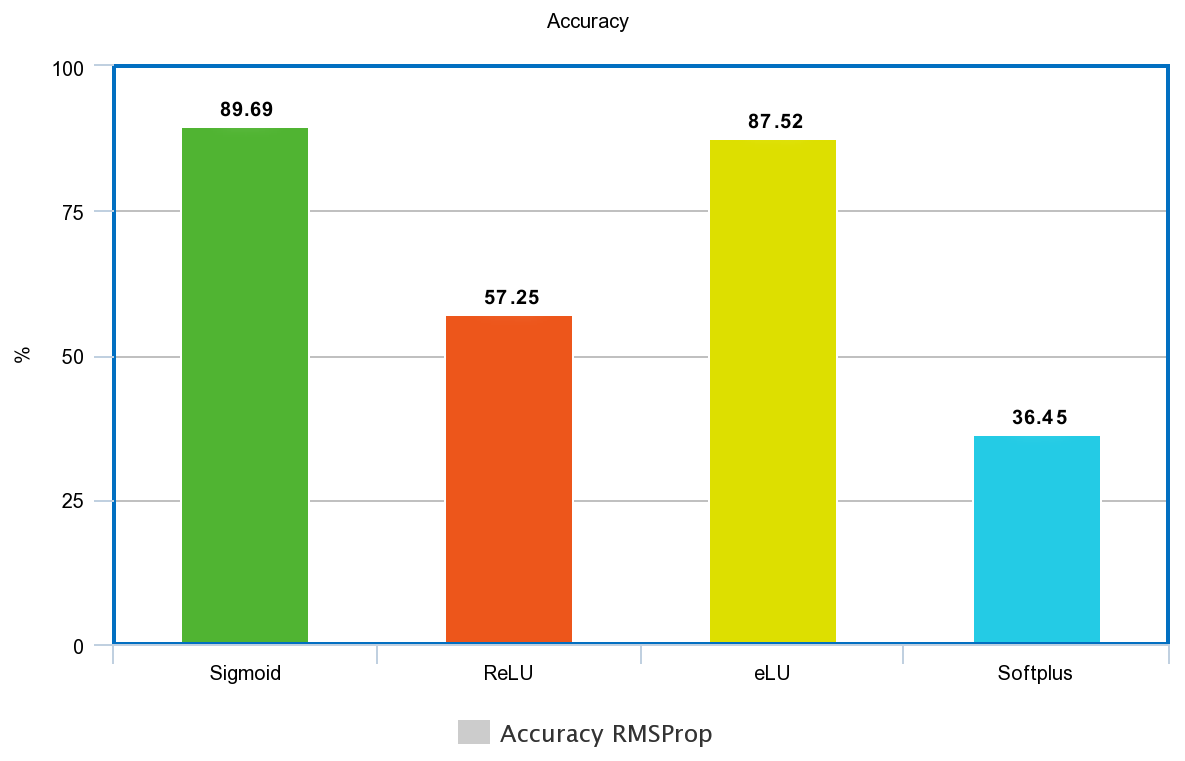
\includegraphics[width=13cm]{accuracy_rmsprop_greedy.png}
\caption{ Accuracy of RMSProp Optimizer for different activation functions}
\label{fig:accuracy_rmsprop_greedy}
\end{figure}
In the table \ref{confusion_rmsprop} we can see that sigmoid activation function has better chances of identifying different classes of attacks
\begin{table}[ht]
\centering
\captionsetup{justification=centering,margin=2cm}
\begin{tabular}{|c|c|c|c|c|c|}
\hline
\textbf{Attack Types} & \textbf{Total Samples} & \textbf{Sigmoid} & \textbf{ReLu} & \textbf{eLu} & \textbf{Softplus} \\ \hline
\textbf{Normal}       & 67342                  & 60465                     & 61945         & 56884        & 0             \\ \hline
\textbf{DoS}          & 45927                  & 43699          		       & 0                  & 0         & 45927             \\ \hline
\textbf{Probe}        & 11656                  & 8156           		  & 9840         & 8365         & 0              \\ \hline
\textbf{U2R}          & 995                    & 662              		& 340           & 926          & 0               \\ \hline
\textbf{R2L}          & 52                     & 13               		& 0            & 0           & 0                \\ \hline
\end{tabular}
\caption{Number of samples correctly identified for RMSProp Optimizer with different Activation functions}
\label{confusion_rmsprop}
\end{table}
\clearpage
\subsubsection{Sigmoid Activation}

\begin{table}[ht]
\centering
\captionsetup{justification=centering,margin=2cm}
\begin{tabular}{|c|c|c|c|c|}
\hline
\multicolumn{1}{|c|}{\textbf{Attack Type}} & \multicolumn{1}{c|}{\textbf{Precision}} & \multicolumn{1}{c|}{\textbf{Recall}} & \multicolumn{1}{c|}{\textbf{F1-Score}} \\ \hline
\textbf{Normal}        & 0.9266                                   & 0.8979                                & 0.9120                                                                  \\ \hline
\textbf{DoS}           & 0.9596                                  & 0.9515                                &  0.9555                                                                    \\ \hline
\textbf{Probe}         & 0.6807                                  & 0.6997                                & 0.6901                                                                  \\ \hline
\textbf{U2R}           & 0.2220                                    & 0.6653                                & 0.3329                                                                   \\ \hline
\textbf{R2L}           & 0.0607                                      & 0.2500                                   & 0.0977                                                            \\ \hline         \end{tabular}
\caption{Precision, Recall, and F1 Score of Stacked Autoencoder with RMSProp Optimizer for Sigmoid Activation}
\label{prf1_rmsprop_sigmoid_auto}
\end{table}

\subsubsection{ReLU Activation}
\begin{table}[ht]
\centering
\captionsetup{justification=centering,margin=2cm}
\begin{tabular}{|c|c|c|c|c|}
\hline
\multicolumn{1}{|c|}{\textbf{Attack Type}} & \multicolumn{1}{c|}{\textbf{Precision}} & \multicolumn{1}{c|}{\textbf{Recall}} & \multicolumn{1}{c|}{\textbf{F1-Score}} \\ \hline
\textbf{Normal}        & 0.9010                                   & 0.9199                                & 0.9103                                                                  \\ \hline
\textbf{DoS}           & 0.0000                                  & 0.0000                                &  0.0000                                                                    \\ \hline
\textbf{Probe}         & 0.1772                                  & 0.8442                                & 0.2929                                                                  \\ \hline
\textbf{U2R}           & 0.2013                                    & 0.3417                                & 0.2534                                                                   \\ \hline
\textbf{R2L}           & 0.0000                                      & 0.0000                                   & 0.0000                                                            \\ \hline         \end{tabular}
\caption{Precision, Recall, and F1 Score of Stacked Autoencoder with RMSProp Optimizer for ReLU Activation}
\label{prf1_rmsprop_relu_auto}
\end{table}

\subsubsection{eLU Activation}

\begin{table}[ht]
\centering
\captionsetup{justification=centering,margin=2cm}
\begin{tabular}{|c|c|c|c|c|}
\hline
\multicolumn{1}{|c|}{\textbf{Attack Type}} & \multicolumn{1}{c|}{\textbf{Precision}} & \multicolumn{1}{c|}{\textbf{Recall}} & \multicolumn{1}{c|}{\textbf{F1-Score}} \\ \hline
\textbf{Normal}        & 0.9538                                   & 0.8447                                & 0.8960                                                                  \\ \hline
\textbf{DoS}           & 0.9656                                  & 0.9597                                &  0.9627                                                                    \\ \hline
\textbf{Probe}         & 0.6481                                  & 0.7177                                & 0.6811                                                                  \\ \hline
\textbf{U2R}           & 0.1190                                    & 0.9307                                & 0.2111                                                                   \\ \hline
\textbf{R2L}           & 0.0000                                      & 0.0000                                   & 0.0000                                                            \\ \hline         \end{tabular}
\caption{Precision, Recall, and F1 Score of Stacked Autoencoder with RMSProp Optimizer for eLU Activation}
\label{prf1_rmsprop_elu_auto}
\end{table}
\clearpage
\subsubsection{Softplus Activation}
\begin{table}[ht]
\centering
\captionsetup{justification=centering,margin=2cm}
\begin{tabular}{|c|c|c|c|c|}
\hline
\multicolumn{1}{|c|}{\textbf{Attack Type}} & \multicolumn{1}{c|}{\textbf{Precision}} & \multicolumn{1}{c|}{\textbf{Recall}} & \multicolumn{1}{c|}{\textbf{F1-Score}} \\ \hline
\textbf{Normal}        & 0.0000                                   & 0.0000                                & 0.0000                                                                  \\ \hline
\textbf{DoS}           & 0.3646                                  & 1.0000                                &  0.5343                                                                    \\ \hline
\textbf{Probe}         & 0.0000                                  & 0.0000                                & 0.0000                                                                  \\ \hline
\textbf{U2R}           & 0.0000                                    & 0.0000                                & 0.0000                                                                   \\ \hline
\textbf{R2L}           & 0.0000                                      & 0.0000                                   & 0.0000                                                            \\ \hline         \end{tabular}
\caption{Precision, Recall, and F1 Score of Stacked Autoencoder with RMSProp Optimizer for Softplus Activation}
\label{prf1_rmsprop_elu_auto}
\end{table}



\subsection {Stochastic Gradient Descent Optimizer}
\begin{figure}[ht]
\centering
\captionsetup{justification=centering,margin=2cm}
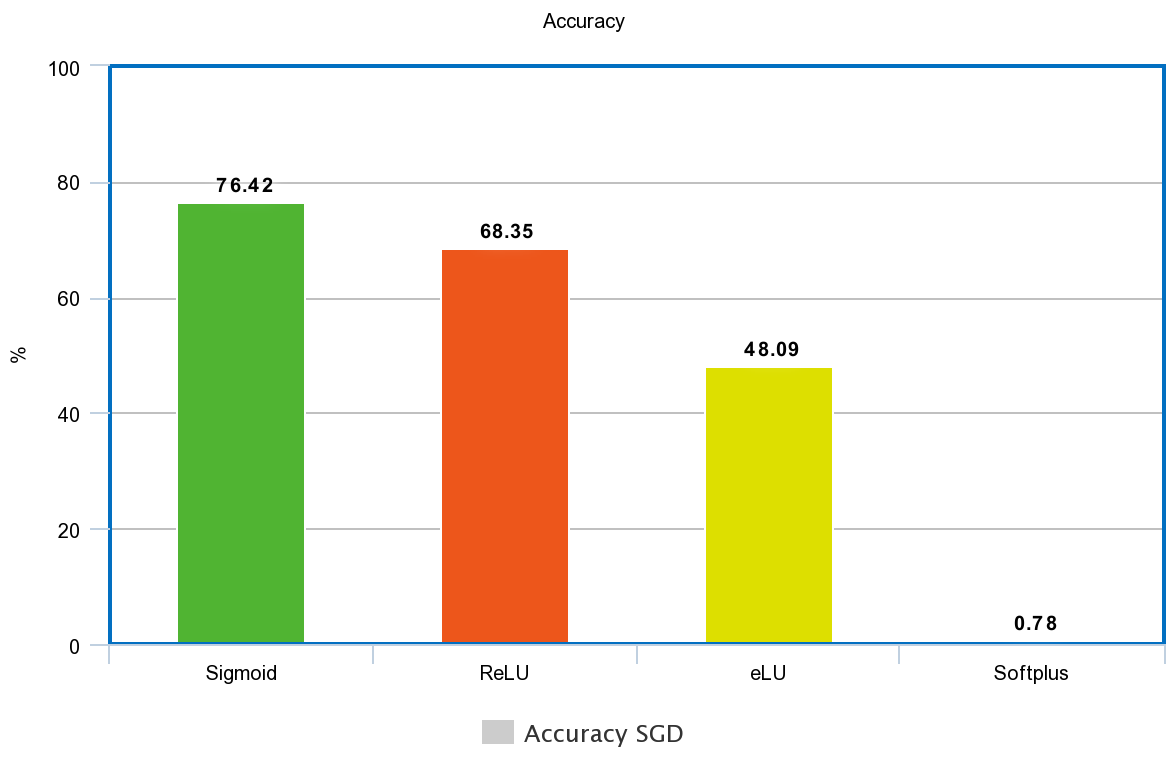
\includegraphics[width=13cm]{accuracy_SGD_greedy.png}
\caption{ Accuracy of Stochastic Gradient Descent Optimizer for different activation functions}
\label{fig:accuracy_sgd_greedy}
\end{figure}

The number of records identified by the Stochastic Gradient Descent Optimizer is in table \ref{confusion_sgd_greedy} and it is clear from that table that \textit{ReLU and eLU} activation function works better with Stochastic Gradient Descent Optimizer. \\ \par
\clearpage
\begin{table}[ht]
\centering
\captionsetup{justification=centering,margin=2cm}
\begin{tabular}{|c|c|c|c|c|c|}
\hline
\textbf{Attack Types} & \textbf{Total Samples} & \textbf{Sigmoid} & \textbf{ReLu} & \textbf{eLu} & \textbf{Softplus} \\ \hline
\textbf{Normal}       & 67342                  & 54189                     & 40123         & 53659              & 0             \\ \hline
\textbf{DoS}          & 45927                  & 42080          		       & 44038        &0         			& 0             \\ \hline
\textbf{Probe}        & 11656                  & 3           			      & 1550           & 6615        		 & 0              \\ \hline
\textbf{U2R}          & 995                      & 0              				& 395           	 & 317                 & 995               \\ \hline
\textbf{R2L}          & 52                          & 0               		          & 1            	 & 0           		 & 0                \\ \hline
\end{tabular}
\caption{Number of samples correctly identified for Stochastic Gradient Descent Optimizer with different Activation functions}
\label{confusion_sgd_greedy}
\end{table}

\subsubsection{Sigmoid Activation}

\begin{table}[ht]
\centering
\captionsetup{justification=centering,margin=2cm}
\begin{tabular}{|c|c|c|c|c|}
\hline
\multicolumn{1}{|c|}{\textbf{Attack Type}} & \multicolumn{1}{c|}{\textbf{Precision}} & \multicolumn{1}{c|}{\textbf{Recall}} & \multicolumn{1}{c|}{\textbf{F1-Score}} \\ \hline
\textbf{Normal}        & 0.8429                                   & 0.8047                                & 0.8234                                                                  \\ \hline
\textbf{DoS}           & 0.6828                                  & 0.9162                                &  0.7825                                                                    \\ \hline
\textbf{Probe}         & 0.7500                                  & 0.0003                                & 0.0005                                                                  \\ \hline
\textbf{U2R}           & 0.0000                                    & 0.0000                                & 0.0000                                                                   \\ \hline
\textbf{R2L}           & 0.0000                                      & 0.0000                                   & 0.0000                                                            \\ \hline         \end{tabular}
\caption{Precision, Recall, and F1 Score of Stacked Autoencoder with Stochastic Gradient Descent Optimizer for Sigmoid Activation}
\label{prf1_sgd_sigmoid_auto}
\end{table}

\subsubsection{ReLU Activation}
\begin{table}[ht]
\centering
\captionsetup{justification=centering,margin=2cm}
\begin{tabular}{|c|c|c|c|c|}
\hline
\multicolumn{1}{|c|}{\textbf{Attack Type}} & \multicolumn{1}{c|}{\textbf{Precision}} & \multicolumn{1}{c|}{\textbf{Recall}} & \multicolumn{1}{c|}{\textbf{F1-Score}} \\ \hline
\textbf{Normal}        & 0.9596                                   & 0.5958                                & 0.7352                                                                  \\ \hline
\textbf{DoS}           & 0.6363                                  & 0.9589                                &  0.7649                                                                    \\ \hline
\textbf{Probe}         & 0.1980                                  & 0.1330                                & 0.1591                                                                  \\ \hline
\textbf{U2R}           & 0.0556                                    & 0.3970                                & 0.0975                                                                   \\ \hline
\textbf{R2L}           & 0.0714                                      & 0.0192                                   & 0.0303                                                            \\ \hline         \end{tabular}
\caption{Precision, Recall, and F1 Score of Stacked Autoencoder with Stochastic Gradient Descent Optimizer for ReLU Activation}
\label{prf1_sgd_relu_auto}
\end{table}
\clearpage
\subsubsection{eLU Activation}

\begin{table}[ht]
\centering
\captionsetup{justification=centering,margin=2cm}
\begin{tabular}{|c|c|c|c|c|}
\hline
\multicolumn{1}{|c|}{\textbf{Attack Type}} & \multicolumn{1}{c|}{\textbf{Precision}} & \multicolumn{1}{c|}{\textbf{Recall}} & \multicolumn{1}{c|}{\textbf{F1-Score}} \\ \hline
\textbf{Normal}        & 0.7487                                   & 0.7968                                & 0.7720                                                                  \\ \hline
\textbf{DoS}           & 0.0000                                  & 0.0000                                &  0.0000                                                                    \\ \hline
\textbf{Probe}         & 0.3399                                  & 0.5675                                & 0.4252                                                                  \\ \hline
\textbf{U2R}           & 0.0627                                    & 0.3186                                & 0.1048                                                                   \\ \hline
\textbf{R2L}           & 0.0000                                      & 0.0000                                   & 0.0000                                                            \\ \hline         \end{tabular}
\caption{Precision, Recall, and F1 Score of Stacked Autoencoder with Stochastic Gradient Descent Optimizer for eLU Activation}
\label{prf1_sgd_elu_auto}
\end{table}

\subsubsection{Softplus Activation}
\begin{table}[ht]
\centering
\captionsetup{justification=centering,margin=2cm}
\begin{tabular}{|c|c|c|c|c|}
\hline
\multicolumn{1}{|c|}{\textbf{Attack Type}} & \multicolumn{1}{c|}{\textbf{Precision}} & \multicolumn{1}{c|}{\textbf{Recall}} & \multicolumn{1}{c|}{\textbf{F1-Score}} \\ \hline
\textbf{Normal}        & 0.0000                                   & 0.0000                                & 0.0000                                                                  \\ \hline
\textbf{DoS}           & 0.0000                                  & 0.0000                                &  0.0000                                                                    \\ \hline
\textbf{Probe}         & 0.0000                                  & 0.0000                                & 0.0000                                                                  \\ \hline
\textbf{U2R}           & 0.0079                                    & 1.0000                                & 0.0157                                                                   \\ \hline
\textbf{R2L}           & 0.0000                                      & 0.0000                                   & 0.0000                                                            \\ \hline         \end{tabular}
\caption{Precision, Recall, and F1 Score of Stacked Autoencoder with Stochastic Gradient Descent Optimizer for Softplus Activation}
\label{prf1_rmsprop_elu_auto}
\end{table}

\clearpage

\subsection {Momentum Optimizer}
\begin{figure}[ht]
\centering
\captionsetup{justification=centering,margin=2cm}
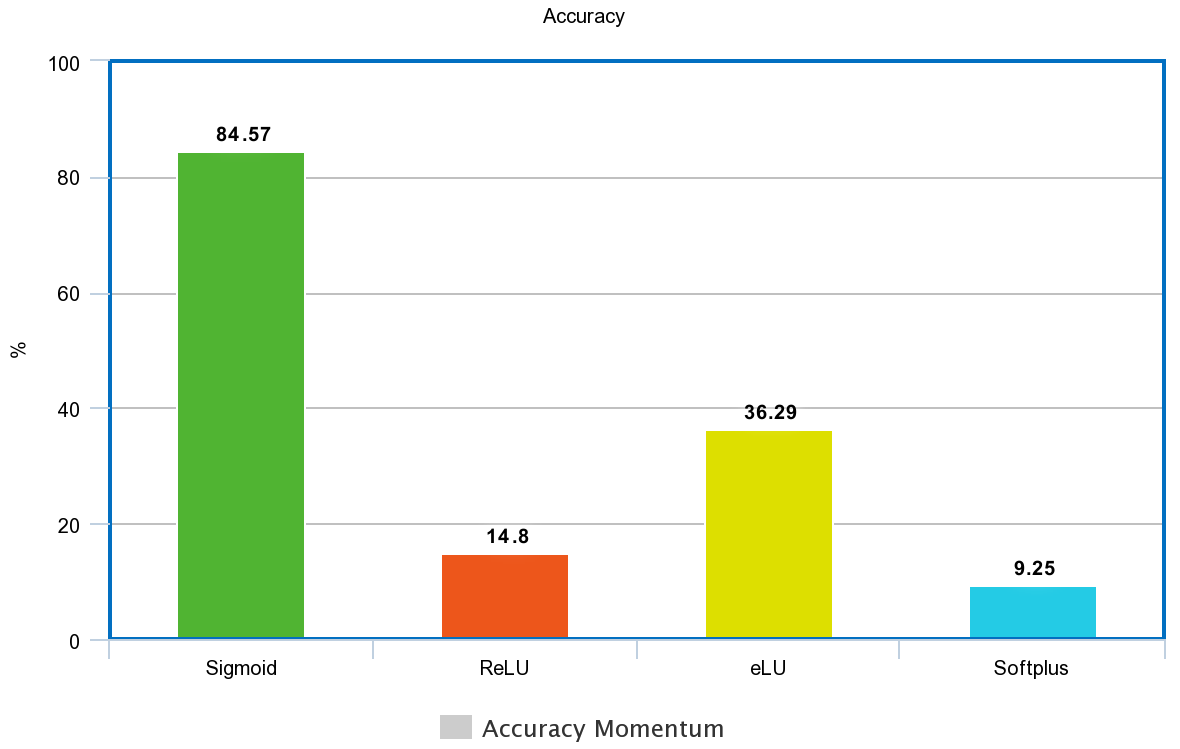
\includegraphics[width=13cm]{accuracy_momentum_greedy.png}
\caption{ Accuracy of Momentum Optimizer for different activation functions}
\label{fig:accuracy_mom_greedy}
\end{figure}

\begin{table}[ht]
\centering
\captionsetup{justification=centering,margin=2cm}
\begin{tabular}{|c|c|c|c|c|c|}
\hline
\textbf{Attack Types} & \textbf{Total Samples} & \textbf{Sigmoid} & \textbf{ReLu} & \textbf{eLu} & \textbf{Softplus} \\ \hline
\textbf{Normal}       & 67342                  & 58606                           & 18267         & 462                           & 0             \\ \hline
\textbf{DoS}          & 45927                  & 42619          		       & 0                 &44841         			  & 0             \\ \hline
\textbf{Probe}        & 11656                  & 5316           			      & 0                  & 0        		 			& 11656            \\ \hline
\textbf{U2R}          & 995                      & 0             		      & 380           	 & 414                			  & 0               \\ \hline
\textbf{R2L}          & 52                          & 0               		            & 2            	 & 0           		            & 0                \\ \hline
\end{tabular}
\caption{Number of samples correctly identified for Momentum Optimizer with different Activation functions}
\label{confusion_mom}
\end{table}
The classification of attacks is not satisfactory with Momentum optimizer, however it was able to identify some records with sigmoid activation function.\\ \par

The \textit{Precision, Recall} and \textit{F-Measure} values for Momentum Optimizer is in the following section.\\ \par
\clearpage
\subsubsection{Sigmoid Activation}
\begin{table}[ht]
\centering
\captionsetup{justification=centering,margin=2cm}
\begin{tabular}{|c|c|c|c|c|}
\hline
\multicolumn{1}{|c|}{\textbf{Attack Type}} & \multicolumn{1}{c|}{\textbf{Precision}} & \multicolumn{1}{c|}{\textbf{Recall}} & \multicolumn{1}{c|}{\textbf{F1-Score}} \\ \hline
\textbf{Normal}        & 0.8622                                   & 0.8703                                & 0.8662                                                                  \\ \hline
\textbf{DoS}           & 0.8232                                  & 0.9280                                &  0.8725                                                                    \\ \hline
\textbf{Probe}         & 0.8530                                  & 0.4561                                & 0.5944                                                                  \\ \hline
\textbf{U2R}           & 0.0000                                    & 0.0000                                & 0.0000                                                                   \\ \hline
\textbf{R2L}           & 0.0000                                      & 0.0000                                   & 0.0000                                                            \\ \hline         \end{tabular}
\caption{Precision, Recall, and F1 Score of Stacked Autoencoder with Momentum Optimizer for Sigmoid Activation}
\label{prf1_mom_sigmoid_auto}
\end{table}

\subsubsection{ReLU Activation}
\begin{table}[ht]
\centering
\captionsetup{justification=centering,margin=2cm}
\begin{tabular}{|c|c|c|c|c|}
\hline
\multicolumn{1}{|c|}{\textbf{Attack Type}} & \multicolumn{1}{c|}{\textbf{Precision}} & \multicolumn{1}{c|}{\textbf{Recall}} & \multicolumn{1}{c|}{\textbf{F1-Score}} \\ \hline
\textbf{Normal}        & 0.3008                                   & 0.2713                                & 0.2853                                                                  \\ \hline
\textbf{DoS}           & 0.0000                                  & 0.0000                                &  0.0000                                                                    \\ \hline
\textbf{Probe}         & 0.0000                                  & 0.0000                                & 0.0000                                                                  \\ \hline
\textbf{U2R}           & 0.0071                                    & 0.3819                                & 0.0139                                                                   \\ \hline
\textbf{R2L}           & 0.0002                                      & 0.0385                                   & 0.0004                                                            \\ \hline         \end{tabular}
\caption{Precision, Recall, and F1 Score of Stacked Autoencoder with Momentum Optimizer for ReLU Activation}
\label{prf1_mom_relu_auto}
\end{table}

\subsubsection{eLU Activation}

\begin{table}[ht]
\centering
\captionsetup{justification=centering,margin=2cm}
\begin{tabular}{|c|c|c|c|c|}
\hline
\multicolumn{1}{|c|}{\textbf{Attack Type}} & \multicolumn{1}{c|}{\textbf{Precision}} & \multicolumn{1}{c|}{\textbf{Recall}} & \multicolumn{1}{c|}{\textbf{F1-Score}} \\ \hline
\textbf{Normal}        & 0.7487                                   & 0.7968                                & 0.7720                                                                  \\ \hline
\textbf{DoS}           & 0.0000                                  & 0.0000                                &  0.0000                                                                    \\ \hline
\textbf{Probe}         & 0.3399                                  & 0.5675                                & 0.4252                                                                  \\ \hline
\textbf{U2R}           & 0.0627                                    & 0.3186                                & 0.1048                                                                   \\ \hline
\textbf{R2L}           & 0.0000                                      & 0.0000                                   & 0.0000                                                            \\ \hline         \end{tabular}
\caption{Precision, Recall, and F1 Score of Stacked Autoencoder with Momentum Optimizer for eLU Activation}
\label{prf1_mom_elu_auto}
\end{table}
\clearpage
\subsubsection{Softplus Activation}
\begin{table}[ht]
\centering
\captionsetup{justification=centering,margin=2cm}
\begin{tabular}{|c|c|c|c|c|}
\hline
\multicolumn{1}{|c|}{\textbf{Attack Type}} & \multicolumn{1}{c|}{\textbf{Precision}} & \multicolumn{1}{c|}{\textbf{Recall}} & \multicolumn{1}{c|}{\textbf{F1-Score}} \\ \hline
\textbf{Normal}        & 0.0000                                   & 0.0000                                & 0.0000                                                                  \\ \hline
\textbf{DoS}           & 0.0000                                  & 0.0000                                &  0.0000                                                                    \\ \hline
\textbf{Probe}         & 0.0925                                  & 1.0000                                & 0.1694                                                                  \\ \hline
\textbf{U2R}           & 0.0000                                    & 0.0000                                & 0.0000                                                                   \\ \hline
\textbf{R2L}           & 0.0000                                      & 0.0000                                   & 0.0000                                                            \\ \hline         \end{tabular}
\caption{Precision, Recall, and F1 Score of Stacked Autoencoder with Momentum Optimizer for Softplus Activation}
\label{prf1_mom_elu_auto}
\end{table}


\clearpage


%%%%%%%%%%%%%%%%%%%%%% Deep Belief Network %%%%%%%%%%%%%%%%%%%%%%%%%%%%%%%%%%%%%%%%%%%%%%%%
\section{Deep Belief Network}\label{sec:dbn_eval}

Deep Belief Networks are made up of stacked Restricted Boltzmann Machine which is explained in \ref{sec:deep_belief_network} and \ref{sec:RBM} \\ 
The accuracy different Optimizers on Sigmoid Activation is given in the Figure \ref{fig:dbn_accu_sigmoid} below.\\ \par
\begin{figure}[ht]
\centering
\captionsetup{justification=centering,margin=2cm}
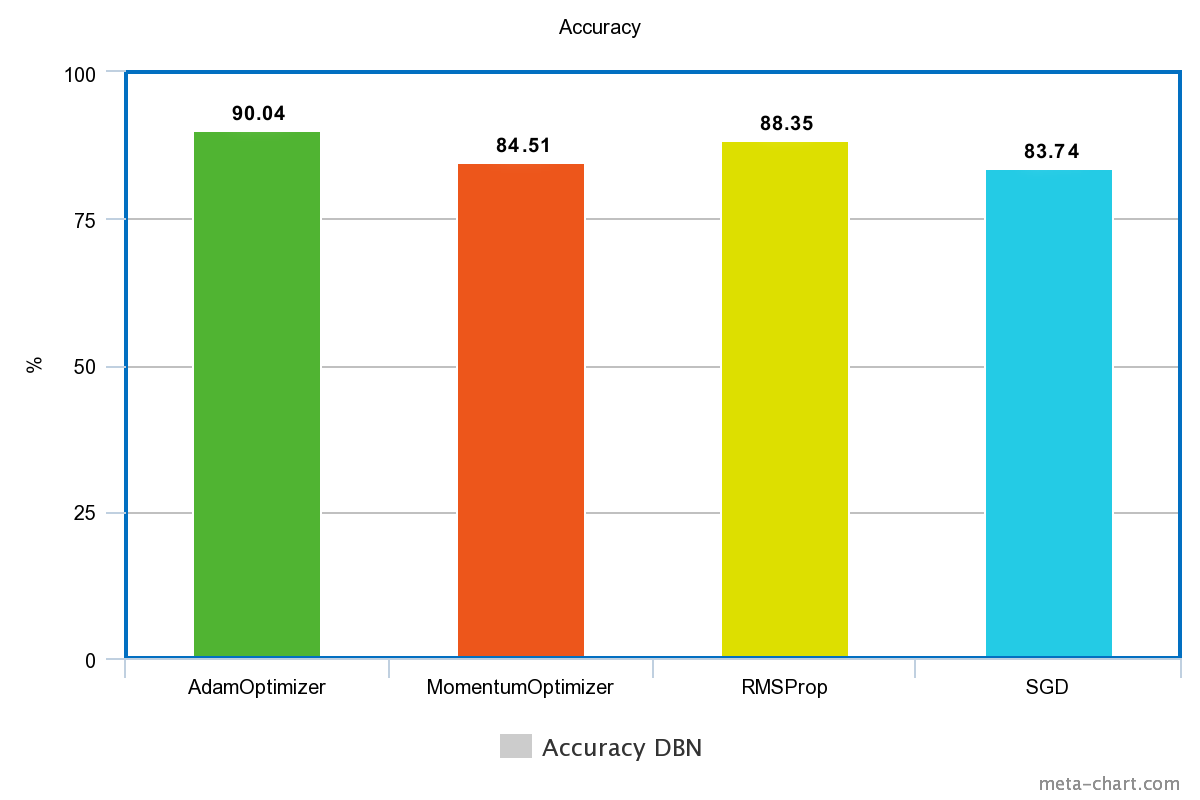
\includegraphics[width=13cm]{DBN_accuracy_optimizer.png}
\caption{ Accuracy of Deep Belief Network with different optimizers for Sigmoid activation }
\label{fig:dbn_accu_sigmoid}
\end{figure}


The parameters used in evaluation of Deep Belief Network (DBN) are different for pre-training phase and fine tuning phase. The following table depicts the parameters used in both the phases.\\ \par

\begin{table}[ht]
\centering
\captionsetup{justification=centering,margin=2cm}
\begin{tabular}{|c|c|c|}
\hline
\textbf{Parameters}          & \textbf{Pre-Training Phase} & \textbf{Fine Tuning Phase} \\ \hline
\textbf{Activation Function} & Sigmoid                     & Sigmoid                    \\ \hline
\textbf{Learning Rate}       & 1.0                         & 0.01                        \\ \hline
\textbf{Batch Size}          & 100                         & 10                         \\ \hline
\textbf{Number of Epochs}    & 10                          & 30                         \\ \hline
\end{tabular}
\caption{Parameters of DBN with Sigmoid Activation}
\label{DBNSigmoidMomentum}
\end{table}
\clearpage
The table \ref{DBN_predicted_attacks} below shows the number of correctly identified attacks types by different optimizers with Sigmoid Activation functions.

\begin{table}[ht]
\centering
\captionsetup{justification=centering,margin=2cm}
\begin{tabular}{|c|c|c|c|c|}
\hline
\textbf{Attack Types} & \textbf{Adam} & \textbf{Mom} & \textbf{RMSProp} & \textbf{SGD} \\ \hline
\textbf{Normal}       & 62141         & 61473        & 59991            & 64251        \\ \hline
\textbf{DoS}          & 43547         & 44008        & 43693            & 41243        \\ \hline
\textbf{Probe}        & 8121          & 961          & 7225             & 0            \\ \hline
\textbf{U2R}          & 101           & 24           & 391              & 0            \\ \hline
\textbf{R2L}          & 0             & 0            & 0                & 0            \\ \hline
\end{tabular}
\caption{Number of samples correctly identified for DBN for different Optimizers with Sigmoid Activation functions}
\label{DBN_predicted_attacks}
\end{table}

The Precision, Recall, and F-Measure for different optimizers with sigmoid activation function is also evaluated in the following section.

\subsubsection{Adam Optimizer}
\begin{table}[ht]
\centering
\captionsetup{justification=centering,margin=2cm}
\begin{tabular}{|c|c|c|c|c|}
\hline
\multicolumn{1}{|c|}{\textbf{Attack Type}} & \multicolumn{1}{c|}{\textbf{Precision}} & \multicolumn{1}{c|}{\textbf{Recall}} & \multicolumn{1}{c|}{\textbf{F1-Score}} \\ \hline
\textbf{Normal}        & 0.9276                                  & 0.9228                               & 0.9252                                                                  \\ \hline
\textbf{DoS}           & 0.9561                                  & 0.9482                                &  0.9521                                                                   \\ \hline
\textbf{Probe}         & 0.6687                                  & 0.6967                                & 0.6824                                                                  \\ \hline
\textbf{U2R}           & 0.0782                                   & 0.1015                                & 0.0883                                                                     \\ \hline
\textbf{R2L}           & 0                                       & 0                                    & 0                                                                          \\ \hline
\end{tabular}
\caption{Precision, Recall, and F1 Score of DBN with Adam Optimizer for Sigmoid Activation}
\label{prf1_adam_dbn}
\end{table}

\subsubsection{Momentum Optimizer}

\begin{table}[ht]
\centering
\captionsetup{justification=centering,margin=2cm}
\begin{tabular}{|c|c|c|c|}
\hline
\textbf{AttackTypes} & \multicolumn{1}{c|}{\textbf{Precision}} & \multicolumn{1}{c|}{\textbf{Recall}} & \multicolumn{1}{c|}{\textbf{F1-Score}} \\ \hline
\textbf{Normal}      & 0.9295                                   & 0.9128                                & 0.9211                                  \\ \hline
\textbf{DoS}         &0.7654                                   & 0.9582                                & 0.8510                                  \\ \hline
\textbf{Probe}       & 0.9431                                   & 0.0824                                & 0.1516                                  \\ \hline
\textbf{U2R}         &0.0182                                   & 0.0241                                & 0.0207                                  \\ \hline
\textbf{R2L}         & 0                                       & 0                                    & 0                                      \\ \hline
\end{tabular}
\caption{Precision, Recall, and F1 Score of DBN with Momentum Optimizer for Sigmoid Activation}
\label{prf1_mom_dbn}
\end{table}
\clearpage
\subsubsection{RMSProp}
\begin{table}[ht]
\centering
\captionsetup{justification=centering,margin=2cm}
\begin{tabular}{|c|c|c|c|}
\hline
\textbf{AttackTypes} & \multicolumn{1}{c|}{\textbf{Precision}} & \multicolumn{1}{c|}{\textbf{Recall}} & \multicolumn{1}{c|}{\textbf{f1-Score}} \\ \hline
\textbf{Normal}      & 0.9224                                  & 0.8908                               & 0.9063                                 \\ \hline
\textbf{DoS}         & 0.9026                                  & 0.9514                               & 0.9263                                 \\ \hline
\textbf{Probe}       & 0.8684                                  & 0.6199                               & 0.7234                                 \\ \hline
\textbf{U2R}         & 0.0931                                  & 0.3930                               & 0.1505                                 \\ \hline
\textbf{R2L}         & 0                                       & 0                                    & 0                                      \\ \hline
\end{tabular}
\caption{Precision, Recall, and F1 Score of DBN with RMSProp Optimizer for Sigmoid Activation}
\label{prf1_rms_dbn}
\end{table}

\subsubsection{Stochastic Gradient Descent Optimizer}
\begin{table}[ht]
\centering
\captionsetup{justification=centering,margin=2cm}
\begin{tabular}{|c|l|l|l|}
\hline
\textbf{AttackTypes} & \multicolumn{1}{c|}{\textbf{Precision}} & \multicolumn{1}{c|}{\textbf{Recall}} & \multicolumn{1}{c|}{\textbf{f1-Score}} \\ \hline
\textbf{Normal}      & 0.8464                                  & 0.9541                               & 0.8970                                 \\ \hline
\textbf{DoS}         & 0.8239                                  & 0.8980                               & 0.8593                                 \\ \hline
\textbf{Probe}       & 0.0000                                  & 0.0000                               & 0.0000                                 \\ \hline
\textbf{U2R}         & 0.0000                                  & 0.0000                               & 0.0000                                 \\ \hline
\textbf{R2L}         & 0                                       & 0                                    & 0                                      \\ \hline
\end{tabular}
\caption{Precision, Recall, and F1 Score of DBN with RMSProp Optimizer for Sigmoid Activation}
\label{prf1_sgd_dbn}
\end{table}
\clearpage
\chapter{Conclusion}

From this project we have concluded that testing our model for different activation function and for different optimization algorithms yields different results on same data. 
\\ \par
The variation in accuracies arises from the nature of the activation functions and the optimization algorithms. As it is seen from the above results that due to non linear nature of data, sigmoid activation yields better results then others. ReLU suffers from knockout problem as the learning rate was a little high, a large gradient can kill a ReLU such that it never gets activated again ever. \\ \par

For Adam optimizer, softplus activation behaves on par with sigmoid activation as seen in Figure \ref{fig:accuracy_adam_greedy}. For RMSProp optimizer, eLU and sigmoid activation yields similar results Figure \ref{fig:accuracy_rmsprop_greedy}. These results can be because of the way these networks were trained. Also we have concluded that training a network in greedily manner affect the results and is more effective in Intrusion Detection Systems. Although this will depend on the dataset in use.\\ \par

The data that we used was clean and preprocessed free of an ambiguity but in real life scenario the data will be corrupt with a lot of ambiguities for which the network has to be robust. Training a denoising autoencoder may be useful in that case. Accuracy is not a good measure in this dataset as the classes are unbalanced. As we can see from the Table \ref{table:test_train},  difference between number of samples in \textit{Normal} and \textit{R2L} class is 67290, so our model cleverly decides to ignore one class completely in favor of high accuracy. Due to this fact we have decided to include other evaluation parameters which gave a broader view of the predictions made by our model. These parameters such as Precision Recall and F-1 Score does not take the whole dataset into account rather it takes each class separately and evaluate the model.   
\\ \par
The case is a lot similar for Deep Belief Network as all the optimizers with sigmoid activation Figure \ref{fig:dbn_accu_sigmoid} shows very similar results.


\begin{thebibliography}{9}
\bibitem{Kaspersky}
Threat Landscape for Industrial Automation System in Second Half of 2016, Kaspersky Lab ICS CERT.
\bibitem{IDS}
INTRUSION DETECTION SYSTEMS;DEFINITION, NEED AND CHALLENGES, SANS Institute 2001,
\bibitem{securityengineering}
Anderson, Ross (2001). Security Engineering: A Guide to Building Dependable Distributed Systems. New York: John Wiley \& Sons. pp. 387–388. ISBN 978-0-471-38922-4.
\bibitem{limitationOfIDS}
Limitations of Network Intrusion Detection, Steve Schupp, December 1, 2000, https://www.giac.org/paper/gsec/235/limitations-network-intrusion-detection/100739
\bibitem{ReLU}
R Hahnloser, R. Sarpeshkar, M A Mahowald, R. J. Douglas, H.S. Seung (2000). Digital selection and analogue amplification coexist in a cortex-inspired silicon circuit. Nature. 405. pp. 947–951.
\bibitem{ELU}
Djork-Arné Clevert, Thomas Unterthiner, Sepp Hochreiter, latest version 22 Feb 2016 (v5).Fast and Accurate Deep Network Learning by Exponential Linear Units (ELUs). arXiv:1511.07289 [cs.LG]
\bibitem{unsupervised}
Goodfellow, Ian J.; Pouget-Abadie, Jean; Mirza, Mehdi; Xu, Bing; Warde-Farley, David; Ozair, Sherjil; Courville, Aaron; Bengio, Yoshua (2014). "Generative Adversarial Networks". arXiv:1406.2661
\bibitem{momentum}
On the momentum term in gradient descent learning algorithms, NingQian, Qinghua Hu, Yun Wang, Zongxia Xie, Pengfei Zhu, Daren Yu
Center for Neurobiology and Behavior, Columbia University, 722 W. 168th Street, New York, NY 10032, USA
\bibitem{OptimizerGeneral}
An overview of gradient descent optimization algorithms, Sebastian Ruder, Cited from: arXiv:1609.04747v2  
\bibitem{tensorflow_paper}
Large-Scale Machine Learning on Heterogeneous Distributed Systems, Preliminary White Paper, November 9, 2015
\bibitem{googleSearch}
Jack Clark. Google turning its lucrative web search over to AI machines, 2015,www.bloomberg.com/news/articles/2015-10-26/googleturning-its-lucrative-web-search-over-to-ai-machines.
\bibitem{challenge1}
 Improving DNNs for LVCSR using rectified linear units and dropout, George E. Dahl, Tara N. Sainath, Geoffrey E. Hinton, 2013
 \bibitem{challenge2}
 A Practical Guide to Training Restricted Boltzmann Machines, I. Aleksander, M. De Gregorio, F.M.G. França, P.M.V. Lima, H. Morton,January 2009
\bibitem{autoencoder}
D.E. Rumelhart, G.E. Hinton, and R.J. Williams. Learning internal representations by error propagation. In Parallel Distributed Processing. Vol 1: Foundations. MIT Press, Cambridge, MA, 1986.
\bibitem{autoencoder2}
Autoencoders, Unsupervised Learning, and Deep Architectures, Pierre Baldi, Department of Computer Science,University of California, Irvine, 2010
\bibitem{ksparseautoencoder}
Alireza Makhzani, Brendan Frey, k-Sparse Autoencoders, 19 Dec 2013, 	arXiv:1312.5663 [cs.LG]
\bibitem{DBN}
Hinton, G. (2009). "Deep belief networks". Scholarpedia. 4 (5): 5947. doi:10.4249/scholarpedia.5947.
\bibitem{RBM}
Smolensky, Paul (1986). "Chapter 6: Information Processing in Dynamical Systems: Foundations of Harmony Theory" (PDF). In Rumelhart, David E.; McLelland, James L. Parallel Distributed Processing: Explorations in the Microstructure of Cognition, Volume 1: Foundations. MIT Press. pp. 194–281. ISBN 0-262-68053-X.
\bibitem{RBMuses}
Ruslan Salakhutdinov and Geoffrey Hinton (2010). Replicated softmax: an undirected topic model. Neural Information Processing Systems.
\bibitem{Greedy}
Yoshua Bengio, Pascal Lamblin, Dan Popovici, Hugo Larochelle, Greedy Layer-Wise Training of Deep Networks, Dec 2006, University of Montreal. 
\end{thebibliography}
\clearpage

%appendix

\begin{appendices}
  \chapter{Results of Non Greedy Training of Stacked Autoencoder in TFlearn}\label{app:super}
 We started with the implementation of \textit{stacked autoencoder}. The library we first started implementing \textit{stacked autoencoder} in was \textbf{Tflearn}. It is a modular deep learning library built on top of Tensorflow, which is designed to provide higher-level API to Tensorflow in order to provide speed in experimentation.\\ \par

We had build a model using Tflearn, just like Tensorflow it allows device placement for using multiple CPU/GPU. We started with building the network with input layer to be of 41 neurons as that is the number of input features that NSL-KDD has. Secondly we decided on having three hidden layers with 30, 20 and 10 neurons respectively. The next thing was to identify which activation function to use. We had gone with the most popular \textit{Sigmoid} activation as it is widely popular. So for the three layers we used the \textit{Sigmoid} activation. The final layer or the output layer has five neurons as we have to classify the attacks in five different classes namely, \textit{Normal, DoS, Probing, R2L, U2R}, hence we have used 5 neurons in the last layer. The activation function for the last layer is \textit{Softmax}, as stated in section \ref{sec:softmax} \textit{Softmax} is used in multi-class classification.\\ \par

After the network is setup, the next task in hand was to define loss function and optimizer function, a \textit{loss function} will calculate the amount of information or data that is lost in the learning process. \textit{Optimizer} will try and minimize the loss parameter. For the purpose of this model we have used the \textit{categorical cross entropy}, which is square of the difference between the estimated values and the original values. \\ \par
\begin{table}[ht]
\centering
\captionsetup{justification=centering,margin=2cm}
\begin{tabular}{|c|c|}
\hline
\textbf{Parameters} & \textbf{Values} \\ \hline
Learning Rate       & 0.001           \\ \hline
Epochs              & 80              \\ \hline
Batch Size          & 100             \\ \hline
\end{tabular}
\caption{Settings used to evaluate stacked autoencoder in tflearn}
\label{setting_tflearn_autoencoder}
\end{table}
\clearpage
 \section{Adam Optimizer}
 \begin{figure}[h]
\centering
\captionsetup{justification=centering,margin=2cm}
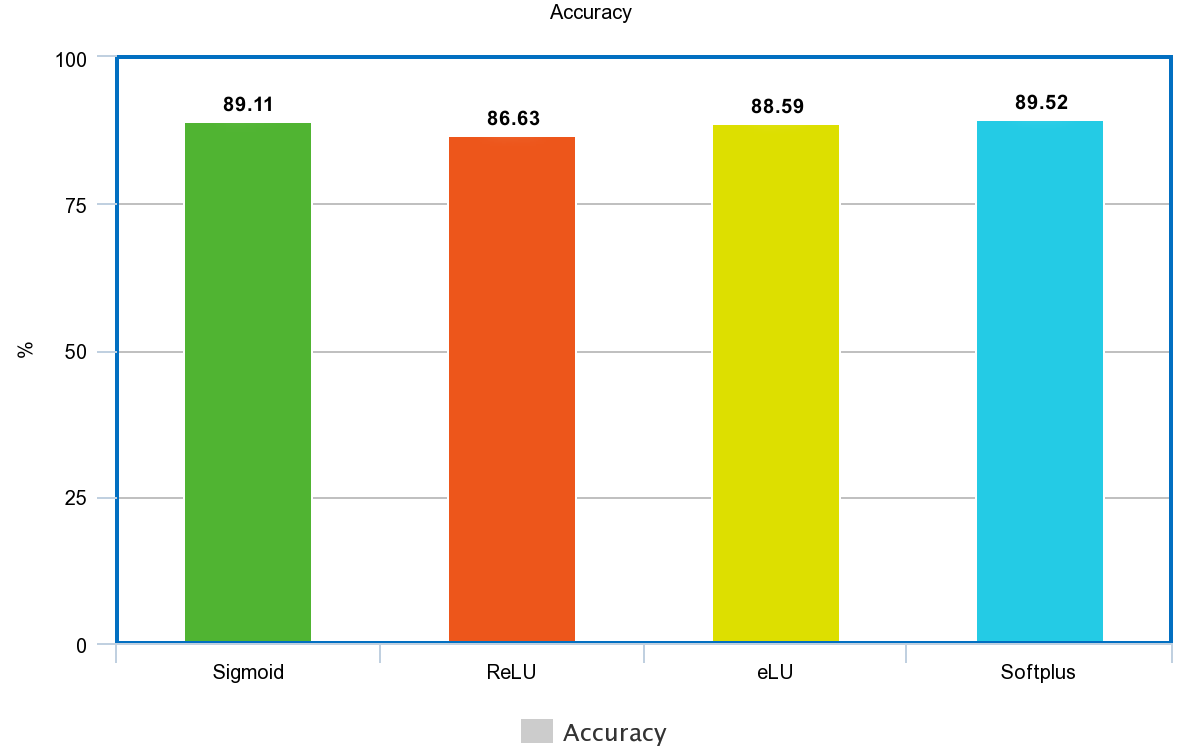
\includegraphics[width=13cm]{accuracy_adam_tflearn.png}
\caption{ Accuracy of Stacked Autoencoder with Adam optimizer for different activation }
\label{fig:acc_adam}
\end{figure}


\begin{table}[h]
\centering
\captionsetup{justification=centering,margin=2cm}
\begin{tabular}{|c|c|c|c|c|c|}
\hline
\textbf{Attack Types} & \textbf{Total Samples} & \textbf{Sigmoid} & \textbf{ReLu} & \textbf{eLu} & \textbf{Softplus} \\ \hline
\textbf{Normal}       & 67342                  & 60102            & 56263         & 60612        & 61729             \\ \hline
\textbf{DoS}          & 45927                  & 43823            & 44161         & 43631        & 43759             \\ \hline
\textbf{Probe}        & 11656                  & 7835             & 7936          & 7187         & 7116              \\ \hline
\textbf{U2R}          & 995                    & 482              & 756           & 153          & 145               \\ \hline
\textbf{R2L}          & 52                     & 20               & 14            & 21           & 29                \\ \hline
\end{tabular}
\caption{Number of samples correctly identified for Adam Optimizer with different Activation functions}
\label{confusion_adam_tflearn}
\end{table}
\clearpage
  The \textit{Precision, Recall and F1-Score} measurement are other parameter we analysed for different activation functions. \\ \par
   \subsection{Sigmoid Activation}
   \begin{table}[h]
	\centering
	\captionsetup{justification=centering,margin=2cm}
	\begin{tabular}{|c|c|c|c|}
	\hline
	\textbf{Attack Types} & \textbf{Precision} & \textbf{Recall} & \textbf{F1-score} \\ \hline
	\textbf{Normal}       & 0.9337             & 0.8925          & 0.9126            \\ \hline
	\textbf{DoS}          & 0.9247             & 0.9542          & 0.9392            \\ \hline
	\textbf{Probe}        & 0.6894             & 0.6721          & 0.6806            \\ \hline
	\textbf{U2R}          & 0.1762             & 0.4844          & 0.2584            \\ \hline
	\textbf{R2L}          & 0.1869             & 0.3846          & 0.2516            \\ \hline
	\end{tabular}
	\caption{Precision Recall and F1-Score Values of Sigmoid Activation for RMSProp Optimizer}
	\label{classification sigmoid adam tflearn}
	\end{table} 
	
	\subsection{ReLu Activation}
   \begin{table}[h]
	\centering
	\captionsetup{justification=centering,margin=2cm}
	\begin{tabular}{|c|c|c|c|}
	\hline
	\textbf{Attack Types} & \textbf{Precision} & \textbf{Recall} & \textbf{F1-score} \\ \hline
	\textbf{Normal}       & 0.9291             & 0.8355          & 0.8798            \\ \hline
	\textbf{DoS}          & 0.9041             & 0.9615          & 0.9319            \\ \hline
	\textbf{Probe}        & 0.6640             & 0.6809          & 0.6723            \\ \hline
	\textbf{U2R}          & 0.1843             & 0.7598          & 0.2966            \\ \hline
	\textbf{R2L}          & 0.0271             & 0.2692          & 0.0492            \\ \hline
	\end{tabular}
	\caption{Precision Recall and F1-Score Values of ReLU Activation for Adam Optimizer}
	\label{classification relu adam tflearn}
	\end{table} 

	\subsection{eLu Activation}
   \begin{table}[h]
	\centering
	\captionsetup{justification=centering,margin=2cm}
	\begin{tabular}{|c|c|c|c|}
	\hline
	\textbf{Attack Types} & \textbf{Precision} & \textbf{Recall} & \textbf{F1-score} \\ \hline
	\textbf{Normal}       & 0.9233             & 0.9001          & 0.9115            \\ \hline
	\textbf{DoS}          & 0.9516             & 0.9500          & 0.9508            \\ \hline
	\textbf{Probe}        & 0.6343             & 0.6166          & 0.6253            \\ \hline
	\textbf{U2R}          & 0.0737             & 0.1538          & 0.0996            \\ \hline
	\textbf{R2L}          & 0.0196             & 0.4038          & 0.0374            \\ \hline
	\end{tabular}
	\caption{Precision Recall and F1-Score Values of elU Activation for Adam Optimizer}
	\label{classification elu adam tflearn}
	\end{table} 
	
	\clearpage
	\subsection{Softplus Activation}
   \begin{table}[ht]
	\centering
	\captionsetup{justification=centering,margin=2cm}
	\begin{tabular}{|c|c|c|c|}
	\hline
	\textbf{Attack Types} & \textbf{Precision} & \textbf{Recall} & \textbf{F1-score} \\ \hline
	\textbf{Normal}       & 0.9383             & 0.9170          & 0.9275            \\ \hline
	\textbf{DoS}          & 0.9524             & 0.9587          & 0.9555            \\ \hline
	\textbf{Probe}        & 0.7142             & 0.6999          & 0.7070            \\ \hline
	\textbf{U2R}          & 0.1176             & 0.1578          & 0.1348            \\ \hline
	\textbf{R2L}          & 0.0223             & 0.5000          & 0.0427            \\ \hline
	\end{tabular}
	\caption{Precision Recall and F1-Score Values of Softplus Activation for Adam Optimizer}
	\label{classification softplus adam tflearn}
	\end{table} 
	
	
	
%%%% RMSProp Extra%%%%%%%%%%%%%%%%%%%%%%%%%%%%
   \section{RMSProp Optimizer}
   \begin{figure}[h]
\centering
\captionsetup{justification=centering,margin=2cm}
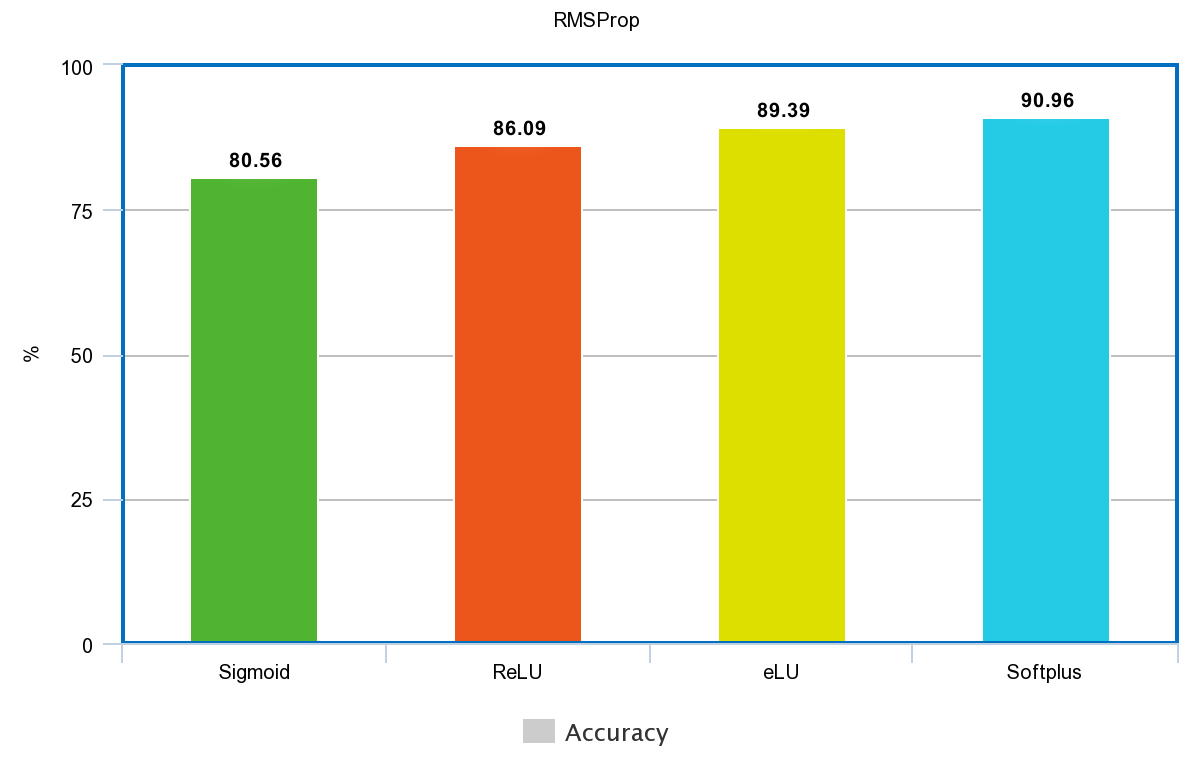
\includegraphics[width=13cm]{accuracy_rmsprop_tflearn.png}
\caption{ Accuracy of Stacked Autoencoder with RMSProp optimizer for different activation }
\label{fig:acc_rms}
\end{figure}
\clearpage
\begin{table}[h]
\centering
\captionsetup{justification=centering,margin=2cm}
\begin{tabular}{|c|c|c|c|c|c|}
\hline
\textbf{Attack Types} & \textbf{Total Samples} & \textbf{Sigmoid} & \textbf{ReLu} & \textbf{eLu} & \textbf{Softplus} \\ \hline
\textbf{Normal}       & 67342                  & 49217            & 57898         & 60346        & 63140             \\ \hline
\textbf{DoS}          & 45927                  & 43393            & 43364         & 43711        & 43352             \\ \hline
\textbf{Probe}        & 11656                  & 8015             & 6277          & 7937         & 7886              \\ \hline
\textbf{U2R}          & 995                    & 862              & 912           & 616          & 208               \\ \hline
\textbf{R2L}          & 52                     & 0               & 21            & 8           & 0                \\ \hline
\end{tabular}
\caption{Number of samples correctly identified for RMSProp Optimizer with different Activation functions}
\label{confusion_rms_tflearn}
\end{table}


   \subsection{Sigmoid Activation}
   \begin{table}[h]
	\centering
	\captionsetup{justification=centering,margin=2cm}
	\begin{tabular}{|c|c|c|c|}
	\hline
	\textbf{Attack Types} & \textbf{Precision} & \textbf{Recall} & \textbf{F1-score} \\ \hline
	\textbf{Normal}       & 0.9207             & 0.7309          & 0.8149            \\ \hline
	\textbf{DoS}          & 0.8268             & 0.9448          & 0.8819            \\ \hline
	\textbf{Probe}        & 0.7103             & 0.6876          & 0.6988            \\ \hline
	\textbf{U2R}          & 0.0985             & 0.8663          & 0.1769            \\ \hline
	\textbf{R2L}          & 0.0000             & 0.0000          & 0.0000            \\ \hline
	\end{tabular}
	\caption{Precision Recall and F1-Score Values of Sigmoid Activation for RMSProp Optimizer}
	\label{classification sigmoid rms tflearn}
	\end{table} 
	
	\subsection{ReLu Activation}
   	\begin{table}[h]
		\centering
		\captionsetup{justification=centering,margin=2cm}
		\begin{tabular}{|c|c|c|c|}
		\hline
		\textbf{Attack Types} & \textbf{Precision} & \textbf{Recall} & \textbf{F1-score} \\ \hline
		\textbf{Normal}       & 0.9175             & 0.8598          & 0.8877            \\ \hline
		\textbf{DoS}          & 0.9217             & 0.9442          & 0.9378            \\ \hline
		\textbf{Probe}        & 0.6503             & 0.5385          & 0.5891            \\ \hline
		\textbf{U2R}          & 0.1368             & 0.9166          & 0.2380            \\ \hline
		\textbf{R2L}          & 0.0000             & 0.0000          & 0.0000            \\ \hline
		\end{tabular}
		\caption{Precision Recall and F1-Score Values of ReLU Activation for RMSProp Optimizer}
		\label{classification relu rms tflearn}
		\end{table} 
	\clearpage
	\subsection{eLu Activation}
 	  \begin{table}[h]
		\centering
		\captionsetup{justification=centering,margin=2cm}
		\begin{tabular}{|c|c|c|c|}
		\hline
		\textbf{Attack Types} & \textbf{Precision} & \textbf{Recall} & \textbf{F1-score} \\ \hline
		\textbf{Normal}       & 0.9234             & 0.8961          & 0.9096            \\ \hline
		\textbf{DoS}          & 0.9605             & 0.9517          & 0.9516            \\ \hline
		\textbf{Probe}        & 0.6869             & 0.6809          & 0.6839            \\ \hline
		\textbf{U2R}          & 0.1871             & 0.6191          & 0.2878            \\ \hline
		\textbf{R2L}          & 0.0299             & 0.1538          & 0.0500            \\ \hline
		\end{tabular}
		\caption{Precision Recall and F1-Score Values of eLU Activation for RMSProp Optimizer}
		\label{classification elu rms tflearn}
		\end{table} 
	
	\subsection{Softplus Activation}
 	  \begin{table}[h]
		\centering
		\captionsetup{justification=centering,margin=2cm}
		\begin{tabular}{|c|c|c|c|}
		\hline
		\textbf{Attack Types} & \textbf{Precision} & \textbf{Recall} & \textbf{F1-score} \\ \hline
		\textbf{Normal}       & 0.9329             & 0.9276          & 0.9352            \\ \hline
		\textbf{DoS}          & 0.9302             & 0.9439          & 0.9370            \\ \hline
		\textbf{Probe}        & 0.7940             & 0.6766          & 0.7306            \\ \hline
		\textbf{U2R}          & 0.1190             & 0.9166          & 0.1517            \\ \hline
		\textbf{R2L}          & 0.0000             & 0.2090          & 0.0000            \\ \hline
		\end{tabular}
		\caption{Precision Recall and F1-Score Values of Softplus Activation for RMSProp Optimizer}
		\label{classification softplus rms tflearn}
		\end{table} 
		\clearpage
%%%%%%%%%%SGD EXTRA%%%%%%%%%%%%%%%%%%%%%%%%%%%%%%%%%%%%%
	\section {Stochastic Gradient Descent Optimizer}
	 \begin{figure}[ht]
\centering
\captionsetup{justification=centering,margin=2cm}
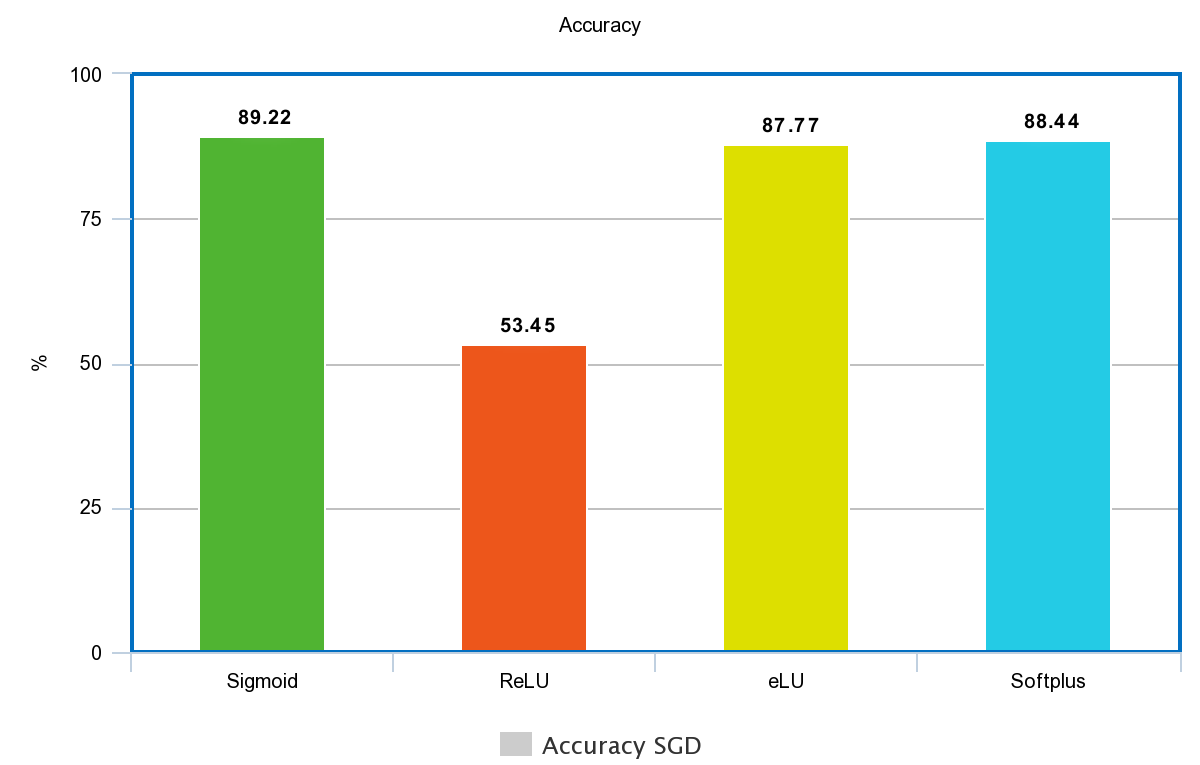
\includegraphics[width=13cm]{accuracy_sgd_tflearn.png}
\caption{ Accuracy of Stacked Autoencoder with Stochastic Gradient Descent optimizer for different activation }
\label{fig:acc_sgd}
\end{figure}
\begin{table}[h]
\centering
\captionsetup{justification=centering,margin=2cm}
\begin{tabular}{|c|c|c|c|c|c|}
\hline
\textbf{Attack Types} & \textbf{Total Samples} & \textbf{Sigmoid} & \textbf{ReLu} & \textbf{eLu} & \textbf{Softplus} \\ \hline
\textbf{Normal}       & 67342                  & 61461            & 67342         & 59815        & 59197             \\ \hline
\textbf{DoS}          & 45927                  & 43505            & 0         & 42755        & 43341             \\ \hline
\textbf{Probe}        & 11656                  & 1441             & 0          & 7163         & 8294              \\ \hline
\textbf{U2R}          & 995                    & 430              & 0           & 845          & 562               \\ \hline
\textbf{R2L}          & 52                     & 22               & 0            & 0           & 26                \\ \hline
\end{tabular}
\caption{Number of samples correctly identified for Stochastic Gradient Descent Optimizer with different Activation functions}
\label{confusion_sgd}
\end{table}
\clearpage
	 \subsection{Sigmoid Activation}
   	\begin{table}[h]
	\centering
	\captionsetup{justification=centering,margin=2cm}
	\begin{tabular}{|c|c|c|c|}
	\hline
	\textbf{Attack Types} & \textbf{Precision} & \textbf{Recall} & \textbf{F1-score} \\ \hline
	\textbf{Normal}       & 0.9221             & 0.9127          & 0.9174            \\ \hline
	\textbf{DoS}          & 0.9611             & 0.9473          & 0.9542            \\ \hline
	\textbf{Probe}        & 0.6916             & 0.5985          & 0.6417            \\ \hline
	\textbf{U2R}          & 0.1194             & 0.4322          & 0.1871            \\ \hline
	\textbf{R2L}          & 0.0601             & 0.4231          & 0.1053            \\ \hline
	\end{tabular}
	\caption{Precision Recall and F1-Score Values of Sigmoid Activation for Stochastic Gradient Descent Optimizer}
	\label{classification sigmoid sgd tflearn}
	\end{table} 

	\subsection{ReLU Activation}
	 \begin{table}[h]
		\centering
		\captionsetup{justification=centering,margin=2cm}
		\begin{tabular}{|c|c|c|c|}
		\hline
		\textbf{Attack Types} & \textbf{Precision} & \textbf{Recall} & \textbf{F1-score} \\ \hline
		\textbf{Normal}       & 0.5346             & 1.0000          & 0.6967            \\ \hline
		\textbf{DoS}          & 0.0000             & 0.0000          & 0.0000            \\ \hline
		\textbf{Probe}        & 0.0000             & 0.0000          & 0.0000            \\ \hline
		\textbf{U2R}          & 0.0000             & 0.0000          & 0.0000            \\ \hline
		\textbf{R2L}          & 0.0000             & 0.0000          & 0.0000            \\ \hline
		\end{tabular}
		\caption{Precision Recall and F1-Score Values of ReLU Activation for Stochastic Gradient Descent Optimizer}
		\label{classification relu sgd tflearn}
		\end{table} 
	
	\subsection{eLu Activation}
 	  \begin{table}[h]
		\centering
		\captionsetup{justification=centering,margin=2cm}
		\begin{tabular}{|c|c|c|c|}
		\hline
		\textbf{Attack Types} & \textbf{Precision} & \textbf{Recall} & \textbf{F1-score} \\ \hline
		\textbf{Normal}       & 0.9422             & 0.8882          & 0.9144            \\ \hline
		\textbf{DoS}          & 0.9569             & 0.9309          & 0.9437            \\ \hline
		\textbf{Probe}        & 0.6208             & 0.6145          & 0.6176            \\ \hline
		\textbf{U2R}          & 0.1349             & 0.8492          & 0.2328            \\ \hline
		\textbf{R2L}          & 0.0000             & 0.0000          & 0.0000            \\ \hline
		\end{tabular}
		\caption{Precision Recall and F1-Score Values of eLU Activation for Stochastic Gradient Descent Optimizer}
		\label{classification elu sgd tflearn}
		\end{table} 
	\clearpage
	\subsection{Softplus Activation}
 	  \begin{table}[h]
		\centering
		\captionsetup{justification=centering,margin=2cm}
		\begin{tabular}{|c|c|c|c|}
		\hline
		\textbf{Attack Types} & \textbf{Precision} & \textbf{Recall} & \textbf{F1-score} \\ \hline
		\textbf{Normal}       & 0.9307             & 0.8791          & 0.9042            \\ \hline
		\textbf{DoS}          & 0.9684             & 0.9437          & 0.9559            \\ \hline
		\textbf{Probe}        & 0.5982             & 0.7116          & 0.6500            \\ \hline
		\textbf{U2R}          & 0.1602             & 0.5648          & 0.2496            \\ \hline
		\textbf{R2L}          & 0.1074             & 0.5000          & 0.1769            \\ \hline
		\end{tabular}
		\caption{Precision Recall and F1-Score Values of Softplus Activation for Stochastic Gradient Descent Optimizer}
		\label{classification softplus sgd tflearn}
		\end{table} 
		
%%%%%%%%%%%%%%%%%%%%%%%Momentum Optimizer%%%%%%%%%%%%%%%%%%%%%%%%%%%%%%%%%%%%%%%%%%%%%%

\section {Momentum Optimizer}
\begin{figure}[ht]
\centering
\captionsetup{justification=centering,margin=2cm}
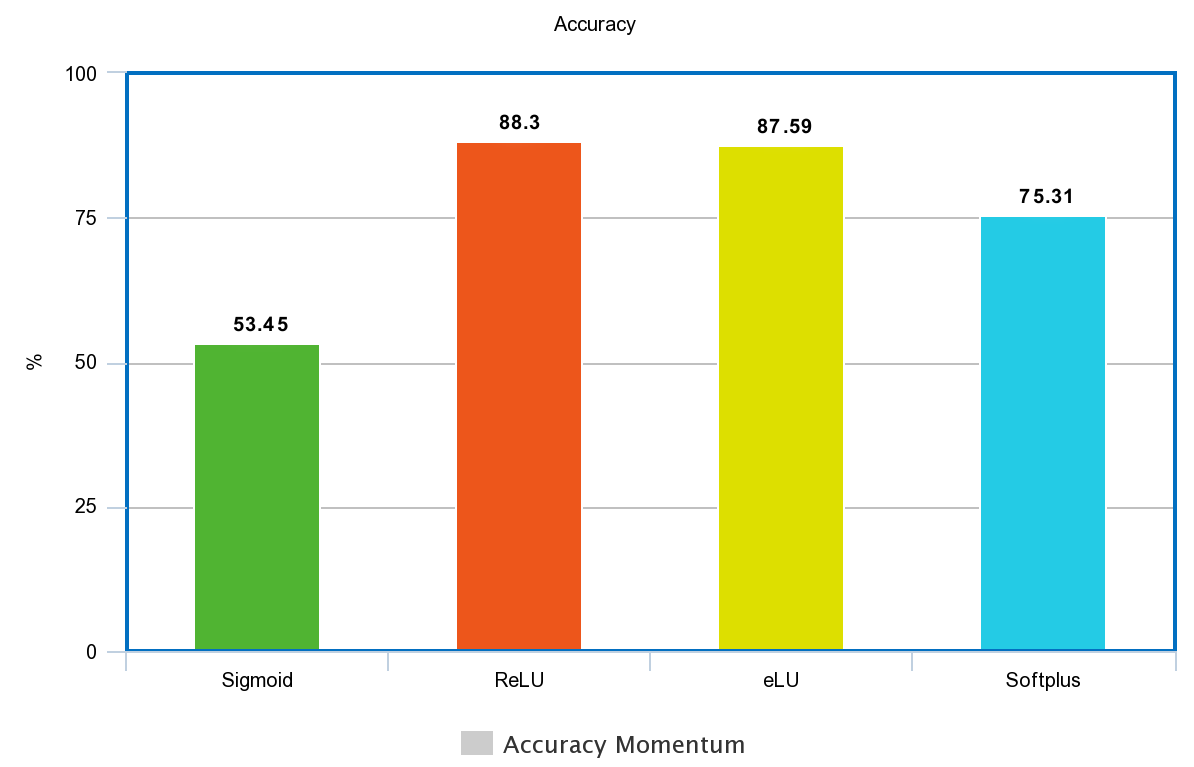
\includegraphics[width=13cm]{accuracy_momentum_tflearn.png}
\caption{ Accuracy of Stacked Autoencoder with Momentum optimizer for different activation }
\label{fig:acc_Momentum}
\end{figure}
\clearpage
\begin{table}[h]
\centering
\captionsetup{justification=centering,margin=2cm}
\begin{tabular}{|c|c|c|c|c|c|}
\hline
\textbf{Attack Types} & \textbf{Total Samples} & \textbf{Sigmoid} & \textbf{ReLu} & \textbf{eLu} & \textbf{Softplus} \\ \hline
\textbf{Normal}       & 67342                  & 67342            & 60660         & 59305        & 43372             \\ \hline
\textbf{DoS}          & 45927                  & 0          		  & 43093         & 43092        & 43024             \\ \hline
\textbf{Probe}        & 11656                  & 0           		  & 6783          & 7104         & 8082              \\ \hline
\textbf{U2R}          & 995                    & 0              		& 689           & 831          & 396               \\ \hline
\textbf{R2L}          & 52                     & 0               		& 13            & 9           & 0                \\ \hline
\end{tabular}
\caption{Number of samples correctly identified for Momentum Optimizer with different Activation functions}
\label{confusion_Momentum}
\end{table}
	 \subsection{Sigmoid Activation}
   	\begin{table}[h]
	\centering
	\captionsetup{justification=centering,margin=2cm}
	\begin{tabular}{|c|c|c|c|}
	\hline
	\textbf{Attack Types} & \textbf{Precision} & \textbf{Recall} & \textbf{F1-score} \\ \hline
	\textbf{Normal}       & 0.5346             & 1.0000          & 0.6967            \\ \hline
	\textbf{DoS}          & 0.0000             & 0.0000          & 0.0000            \\ \hline
	\textbf{Probe}        & 0.0000             & 0.0000          & 0.0000            \\ \hline
	\textbf{U2R}          & 0.0000             & 0.0000          & 0.0000            \\ \hline
	\textbf{R2L}          & 0.0000             & 0.0000          & 0.0000            \\ \hline
	\end{tabular}
	\caption{Precision Recall and F1-Score Values of Sigmoid Activation for Momentum Optimizer}
	\label{classification sigmoid Momentum tflearn}
	\end{table} 
	
	\subsection{ReLU Activation}
	 \begin{table}[h]
		\centering
		\captionsetup{justification=centering,margin=2cm}
		\begin{tabular}{|c|c|c|c|}
		\hline
		\textbf{Attack Types} & \textbf{Precision} & \textbf{Recall} & \textbf{F1-score} \\ \hline
		\textbf{Normal}       & 0.9345             & 0.9008          & 0.9173            \\ \hline
		\textbf{DoS}          & 0.9397             & 0.9383          & 0.9390            \\ \hline
		\textbf{Probe}        & 0.6121             & 0.5819          & 0.5966            \\ \hline
		\textbf{U2R}          & 0.1692             & 0.6925          & 0.2720            \\ \hline
		\textbf{R2L}          & 0.2708             & 0.2500          & 0.2600            \\ \hline
		\end{tabular}
		\caption{Precision Recall and F1-Score Values of ReLU Activation for Momentum Optimizer}
		\label{classification relu Momentum tflearn}
		\end{table} 
	\clearpage
	\subsection{eLu Activation}
 	  \begin{table}[h]
		\centering
		\captionsetup{justification=centering,margin=2cm}
		\begin{tabular}{|c|c|c|c|}
		\hline
		\textbf{Attack Types} & \textbf{Precision} & \textbf{Recall} & \textbf{F1-score} \\ \hline
		\textbf{Normal}       & 0.9530             & 0.8807          & 0.9154            \\ \hline
		\textbf{DoS}          & 0.9075             & 0.9383          & 0.9226            \\ \hline
		\textbf{Probe}        & 0.6039             & 0.6095          & 0.6067            \\ \hline
		\textbf{U2R}          & 0.1863             & 0.8352          & 0.3046            \\ \hline
		\textbf{R2L}          & 0.2812             & 0.1731          & 0.2143            \\ \hline
		\end{tabular}
		\caption{Precision Recall and F1-Score Values of eLU Activation for Momentum Optimizer}
		\label{classification elu Momentum tflearn}
		\end{table} 

	\subsection{Softplus Activation}
 	  \begin{table}[h]
		\centering
		\captionsetup{justification=centering,margin=2cm}
		\begin{tabular}{|c|c|c|c|}
		\hline
		\textbf{Attack Types} & \textbf{Precision} & \textbf{Recall} & \textbf{F1-score} \\ \hline
		\textbf{Normal}       & 0.9619             & 0.6441          & 0.7715            \\ \hline
		\textbf{DoS}          & 0.8974             & 0.9368          & 0.9167            \\ \hline
		\textbf{Probe}        & 0.6199             & 0.6934          & 0.6546            \\ \hline
		\textbf{U2R}          & 0.0199             & 0.3980          & 0.0379            \\ \hline
		\textbf{R2L}          & 0.0000             & 0.0000          & 0.0000            \\ \hline
		\end{tabular}
		\caption{Precision Recall and F1-Score Values of Softplus Activation for Momentum Optimizer}
		\label{classification softplus Momentum tflearn}
		\end{table} 

	
	
	
	





	
%%%%%%%%%%%%%%%%UNSUPERVISED ATUTOENCODER%%%%%%%%%%%%%%%%%%%%%%%	
  \chapter{Results of Non Greedy Training of Stacked Autoencoder in Tensorflow}\label{app:unsuper_tf}
  Just like in \textit{TFlearn}, stacked autoencoder without greedy layer wise pre-training was implemented in \textit{Tensorflow} as well but the number of epoch were increased from 80 to 300 to see if the results gets better or not.\\ \par
  


  \section{Adam Optimizer}
  	\begin{figure}[ht]
	\centering
	\captionsetup{justification=centering,margin=2cm}
	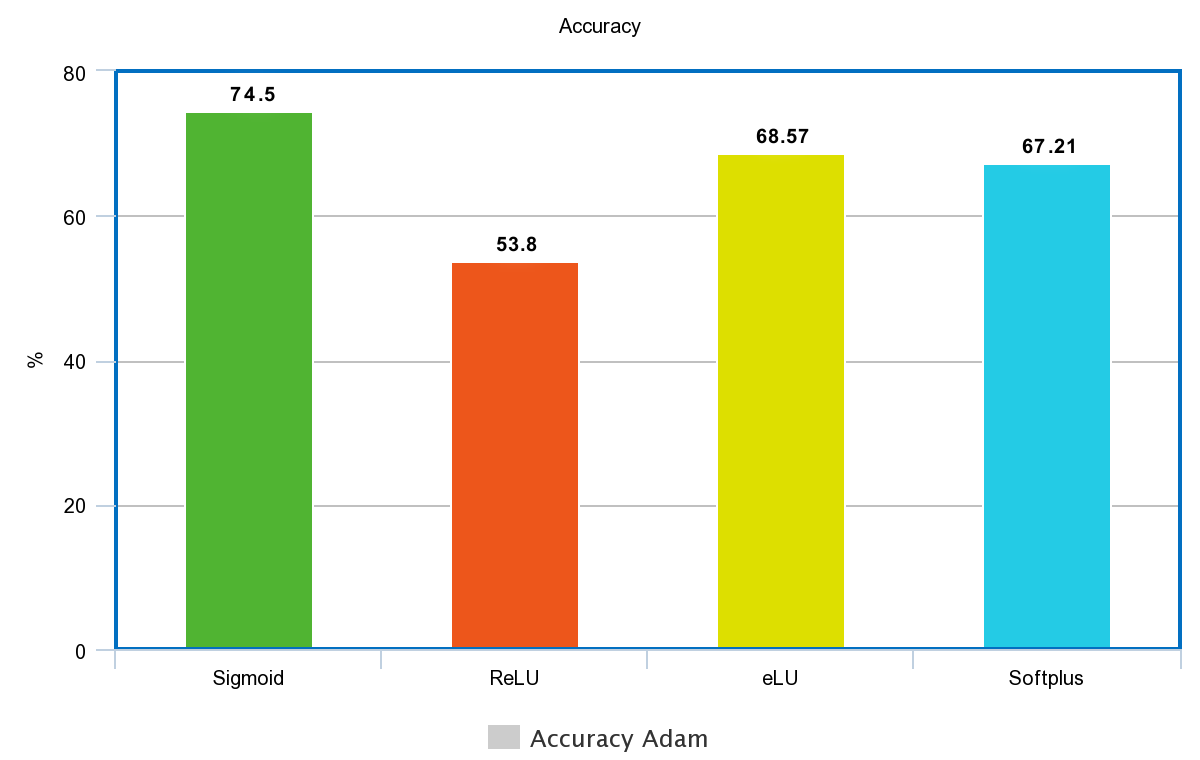
\includegraphics[width=12cm]{Adam_accuracy_tensorflow.png}
	\caption{ Accuracy of Stacked Autoencoder with Adam optimizer for different activation, Unsupervised Learning }
	\label{fig:acc_adam_tf}
	\end{figure}
	
 
	\begin{table}[h]
	\centering
	\captionsetup{justification=centering,margin=2cm}
	\begin{tabular}{|c|c|c|c|c|c|}
	\hline
	\textbf{Attack Types} & \textbf{Total Samples} & \textbf{Sigmoid} & \textbf{ReLu} & \textbf{eLu} & \textbf{Softplus} \\ \hline
	\textbf{Normal}       & 10003                  & 9769            & 9948         & 9943        & 9951           \\ \hline
	\textbf{DoS}          & 7164                  & 5314            & 2180         & 5516        & 5200             \\ \hline
	\textbf{Probe}        & 2421                  & 1491             & 0          & 0         & 0              \\ \hline
	\textbf{U2R}          & 2887                    & 215             & 0           & 0          & 0               \\ \hline
	\textbf{R2L}          & 67                     & 6               & 0            & 0           & 0                \\ \hline
	\end{tabular}
	\caption{Number of samples correctly identified for Adam Optimizer with different Activation functions, Unsupervised Learning}
	\label{confusion_adam_tf}
	\end{table}
  
  As we can see that with \textit{Adam Optimizer}, only the \textit{sigmoid activation} was able to classify correctly different attack types,\text{ ReLU, eLU, and Softpuls} were unable to classify single \textit{Probing, U2R and R2L} attacks.
%%%%%%%%%%%%%%%% sigmoid adam tf %%%%%%%%%%%%%%%%%%%%%%%%%%%%%%	
   \subsection{Sigmoid Activation}
 	 \begin{table}[ht]
		\centering
		\captionsetup{justification=centering,margin=2cm}
		\begin{tabular}{|c|c|c|c|}
		\hline
		\textbf{Attack Types} & \textbf{Precision} & \textbf{Recall} & \textbf{F1-score} \\ \hline
		\textbf{Normal}       & 0.6763             & 0.9766          & 0.7992            \\ \hline
		\textbf{DoS}          & 0.9571             & 0.7418          & 0.8553            \\ \hline
		\textbf{Probe}        & 0.7986             & 0.6159          & 0.6954            \\ \hline
		\textbf{U2R}          & 0.3365             & 0.0745          & 0.1220            \\ \hline
		\textbf{R2L}          & 0.1538             & 0.0896          & 0.1132            \\ \hline
		\end{tabular}
		\caption{Precision Recall and F1-Score Values of Sigmoid Activation for Adam Optimizer, Unsupervised Learning}
		\label{classification sigmoid adam tf}
		\end{table} 
  
  %%%%%%%%%%%%%% Relu adam tf%%%%%%%%%%%%%%%%%%%%%%%%%%%%%%%%%%%%%%%%%%%%%%%%%
  
  \subsection{ReLU Activation}
  \begin{table}[h]
		\centering
		\captionsetup{justification=centering,margin=2cm}
		\begin{tabular}{|c|c|c|c|}
		\hline
		\textbf{Attack Types} & \textbf{Precision} & \textbf{Recall} & \textbf{F1-score} \\ \hline
		\textbf{Normal}       & 0.4934             & 0.9945          & 0.6596            \\ \hline
		\textbf{DoS}          & 0.9160             & 0.3034          & 0.4568            \\ \hline
		\textbf{Probe}        & 0.0000             & 0.0000          & 0.0000            \\ \hline
		\textbf{U2R}          & 0.0000             & 0.0000          & 0.0000            \\ \hline
		\textbf{R2L}          & 0.0000             & 0.0000          & 0.0000            \\ \hline
		\end{tabular}
		\caption{Precision Recall and F1-Score Values of ReLU Activation for Adam Optimizer, Unsupervised Learning}
		\label{classification ReLU adam tf}
		\end{table} 
\clearpage
 %%%%%%%%%%%%%% ELU adam tf %%%%%%%%%%%%%
   \subsection{eLU Activation}
  \begin{table}[h]
		\centering
		\captionsetup{justification=centering,margin=2cm}
		\begin{tabular}{|c|c|c|c|}
		\hline
		\textbf{Attack Types} & \textbf{Precision} & \textbf{Recall} & \textbf{F1-score} \\ \hline
		\textbf{Normal}       & 0.6170             & 0.9940          & 0.7614            \\ \hline
		\textbf{DoS}          & 0.8583             & 0.7700          & 0.8117            \\ \hline
		\textbf{Probe}        & 0.0000             & 0.0000          & 0.0000            \\ \hline
		\textbf{U2R}          & 0.0000             & 0.0000          & 0.0000            \\ \hline
		\textbf{R2L}          & 0.0000             & 0.0000          & 0.0000            \\ \hline
		\end{tabular}
		\caption{Precision Recall and F1-Score Values of eLU Activation for Adam Optimizer, Unsupervised Learning}
		\label{classification eLU adam tf}
		\end{table} 
  
   %%%%%%%%%%%%%% Softplus adam tf %%%%%%%%%%%%%
   \subsection{Softplus Activation}
  \begin{table}[h]
		\centering
		\captionsetup{justification=centering,margin=2cm}
		\begin{tabular}{|c|c|c|c|}
		\hline
		\textbf{Attack Types} & \textbf{Precision} & \textbf{Recall} & \textbf{F1-score} \\ \hline
		\textbf{Normal}       & 0.5814             & 0.9948          & 0.7339            \\ \hline
		\textbf{DoS}          & 0.8583             & 0.7259          & 0.8260            \\ \hline
		\textbf{Probe}        & 0.9582             & 0.0000          & 0.0000            \\ \hline
		\textbf{U2R}          & 0.0000             & 0.0000          & 0.0000            \\ \hline
		\textbf{R2L}          & 0.0000             & 0.0000          & 0.0000            \\ \hline
		\end{tabular}
		\caption{Precision Recall and F1-Score Values of Softplus Activation for Adam Optimizer, Unsupervised Learning}
		\label{classification softplus adam tf}
		\end{table} 
%%%%%%%%%%%%%%%% RMSPROP OPTIMIZER%%%%%%%%%%%%%%%%%%%%%%%%%%%%%%%%%%%%%%%%%%%%%%%%%%\
\clearpage
\section {RMSProp Optimizer}

  	\begin{figure}[ht]
	\centering
	\captionsetup{justification=centering,margin=2cm}
	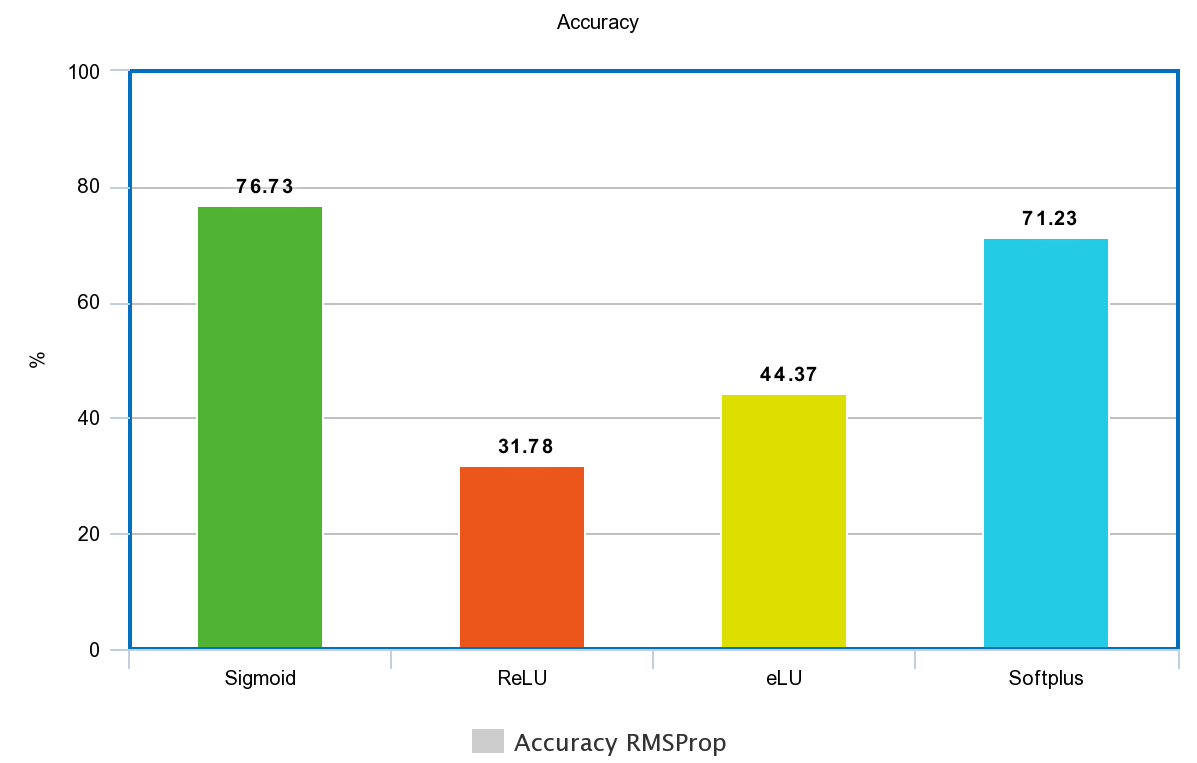
\includegraphics[width=13cm]{RMSprop_accuracy_tensorflow.png}
	\caption{ Accuracy of Stacked Autoencoder with RMSProp optimizer for different activation, Unsupervised Learning }
	\label{fig:acc_RMSProp_tf}
	\end{figure}
	
 
	\begin{table}[h]
	\centering
	\captionsetup{justification=centering,margin=2cm}
	\begin{tabular}{|c|c|c|c|c|c|}
	\hline
	\textbf{Attack Types} & \textbf{Total Samples} & \textbf{Sigmoid} & \textbf{ReLu} & \textbf{eLu} & \textbf{Softplus} \\ \hline
	\textbf{Normal}       & 10003                  & 9662            & 0         & 10003        & 9756           \\ \hline
	\textbf{DoS}          & 7164                  & 5905            & 7164         & 0        & 4805             \\ \hline
	\textbf{Probe}        & 2421                  & 1521             & 0          & 0         & 1497              \\ \hline
	\textbf{U2R}          & 2887                    & 205             & 0           & 0          & 0               \\ \hline
	\textbf{R2L}          & 67                     & 5               & 0            & 0           & 0                \\ \hline
	\end{tabular}
	\caption{Number of samples correctly identified for RMSProp Optimizer with different Activation functions, Unsupervised Learning}
	\label{confusion_RMSProp_tf}
	\end{table}
  
  As we can see that with \textit{Adam Optimizer}, only the \textit{sigmoid activation} was able to classify correctly different attack types,\text{ ReLU, eLU, and Softpuls} were unable to classify single \textit{Probing, U2R and R2L} attacks.
%%%%%%%%%%%%%%%% sigmoid adam tf %%%%%%%%%%%%%%%%%%%%%%%%%%%%%%	
   \clearpage
   \subsection{Sigmoid Activation}
 	 \begin{table}[ht]
		\centering
		\captionsetup{justification=centering,margin=2cm}
		\begin{tabular}{|c|c|c|c|}
		\hline
		\textbf{Attack Types} & \textbf{Precision} & \textbf{Recall} & \textbf{F1-score} \\ \hline
		\textbf{Normal}       & 0.6763             & 0.9766          & 0.7992            \\ \hline
		\textbf{DoS}          & 0.9571             & 0.7418          & 0.8553            \\ \hline
		\textbf{Probe}        & 0.7986             & 0.6159          & 0.6954            \\ \hline
		\textbf{U2R}          & 0.3365             & 0.0745          & 0.1220            \\ \hline
		\textbf{R2L}          & 0.1538             & 0.0896          & 0.1132            \\ \hline
		\end{tabular}
		\caption{Precision Recall and F1-Score Values of Sigmoid Activation for RMSProp Optimizer, Unsupervised Learning}
		\label{classification sigmoid RMSProp tf}
		\end{table} 
  
  %%%%%%%%%%%%%% Relu adam tf%%%%%%%%%%%%%%%%%%%%%%%%%%%%%%%%%%%%%%%%%%%%%%%%%
  
  \subsection{ReLU Activation}
  \begin{table}[h]
		\centering
		\captionsetup{justification=centering,margin=2cm}
		\begin{tabular}{|c|c|c|c|}
		\hline
		\textbf{Attack Types} & \textbf{Precision} & \textbf{Recall} & \textbf{F1-score} \\ \hline
		\textbf{Normal}       & 0.0000             & 0.0000          & 0.0000            \\ \hline
		\textbf{DoS}          & 0.3178             & 1.0000          & 0.4823            \\ \hline
		\textbf{Probe}        & 0.0000             & 0.0000          & 0.0000            \\ \hline
		\textbf{U2R}          & 0.0000             & 0.0000          & 0.0000            \\ \hline
		\textbf{R2L}          & 0.0000             & 0.0000          & 0.0000            \\ \hline
		\end{tabular}
		\caption{Precision Recall and F1-Score Values of ReLU Activation for RMSProp Optimizer, Unsupervised Learning}
		\label{classification ReLU RMSProp tf}
		\end{table} 

 %%%%%%%%%%%%%% ELU adam tf %%%%%%%%%%%%%
   \subsection{eLU Activation}
  \begin{table}[h]
		\centering
		\captionsetup{justification=centering,margin=2cm}
		\begin{tabular}{|c|c|c|c|}
		\hline
		\textbf{Attack Types} & \textbf{Precision} & \textbf{Recall} & \textbf{F1-score} \\ \hline
		\textbf{Normal}       & 0.4438             & 1.0000          & 0.6148            \\ \hline
		\textbf{DoS}          & 0.0000             & 0.0000          & 0.0000            \\ \hline
		\textbf{Probe}        & 0.0000             & 0.0000          & 0.0000            \\ \hline
		\textbf{U2R}          & 0.0000             & 0.0000          & 0.0000            \\ \hline
		\textbf{R2L}          & 0.0000             & 0.0000          & 0.0000            \\ \hline
		\end{tabular}
		\caption{Precision Recall and F1-Score Values of eLU Activation for RMSProp Optimizer, Unsupervised Learning}
		\label{classification eLU RMSProp tf}
		\end{table} 
  \clearpage
   %%%%%%%%%%%%%% Softplus adam tf %%%%%%%%%%%%%
   \subsection{Softplus Activation}
  \begin{table}[h]
		\centering
		\captionsetup{justification=centering,margin=2cm}
		\begin{tabular}{|c|c|c|c|}
		\hline
		\textbf{Attack Types} & \textbf{Precision} & \textbf{Recall} & \textbf{F1-score} \\ \hline
		\textbf{Normal}       & 0.6362             & 0.9753          & 0.7701            \\ \hline
		\textbf{DoS}          & 0.9850             & 0.6707          & 0.7980            \\ \hline
		\textbf{Probe}        & 0.6428             & 0.6183          & 0.6303            \\ \hline
		\textbf{U2R}          & 0.0000             & 0.0000          & 0.0000            \\ \hline
		\textbf{R2L}          & 0.0000             & 0.0000          & 0.0000            \\ \hline
		\end{tabular}
		\caption{Precision Recall and F1-Score Values of Softplus Activation for RMSProp Optimizer, Unsupervised Learning}
		\label{classification softplus RMSProp tf}
		\end{table} 

 
\clearpage

%%%%%%%%%%%%%%%%%% SGD OPTIMIZER %%%%%%%%%%%%%%%%%%%%%%%%%%%%%%%%%%%%%%%%%%%%%%%%%%%%%


\section{Stochastic Gradient Descent Optimizer}
  	\begin{figure}[ht]
	\centering
	\captionsetup{justification=centering,margin=2cm}
	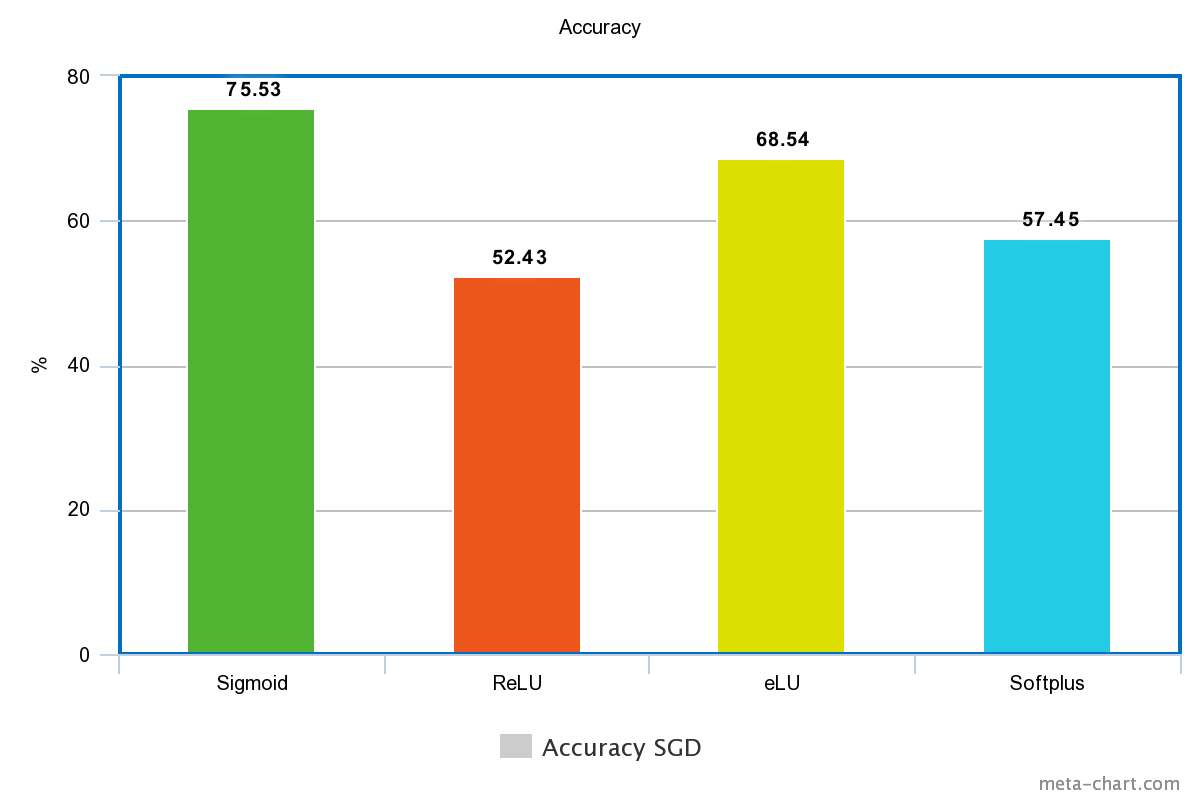
\includegraphics[width=13cm]{SGD_accuracy_tensorflow.png}
	\caption{ Accuracy of Stacked Autoencoder with Stochastic Gradient Descent optimizer for different activation, Unsupervised Learning }
	\label{fig:acc_sgd_tf}
	\end{figure}
	
 
	\begin{table}[h]
	\centering
	\captionsetup{justification=centering,margin=2cm}
	\begin{tabular}{|c|c|c|c|c|c|}
	\hline
	\textbf{Attack Types} & \textbf{Total Samples} & \textbf{Sigmoid} & \textbf{ReLu} & \textbf{eLu} & \textbf{Softplus} \\ \hline
	\textbf{Normal}       & 10003                  & 9696            & 9106         & 9792        & 8802           \\ \hline
	\textbf{DoS}          & 7164                  & 5392            & 2714         & 4524        & 3078             \\ \hline
	\textbf{Probe}        & 2421                  & 1937             & 0          & 1136         & 1071              \\ \hline
	\textbf{U2R}          & 2887                    & 0             & 0           & 0          & 0               \\ \hline
	\textbf{R2L}          & 67                     & 0               & 0            & 0           & 0                \\ \hline
	\end{tabular}
	\caption{Number of samples correctly identified for Stochastic Gradient Descent Optimizer with different Activation functions, Unsupervised Learning}
	\label{confusion_sgd_tf}
	\end{table}
  
  As we can see that with \textit{Adam Optimizer}, only the \textit{sigmoid activation} was able to classify correctly different attack types,\text{ ReLU, eLU, and Softpuls} were unable to classify single \textit{Probing, U2R and R2L} attacks.
%%%%%%%%%%%%%%%% sigmoid adam tf %%%%%%%%%%%%%%%%%%%%%%%%%%%%%%	
   \clearpage
   \subsection{Sigmoid Activation}
 	 \begin{table}[ht]
		\centering
		\captionsetup{justification=centering,margin=2cm}
		\begin{tabular}{|c|c|c|c|}
		\hline
		\textbf{Attack Types} & \textbf{Precision} & \textbf{Recall} & \textbf{F1-score} \\ \hline
		\textbf{Normal}       & 0.6663             & 0.9693          & 0.7897            \\ \hline
		\textbf{DoS}          & 0.9608             & 0.7527          & 0.8441            \\ \hline
		\textbf{Probe}        & 0.8149             & 0.8001          & 0.8074            \\ \hline
		\textbf{U2R}          & 0.0000             & 0.0000          & 0.0000            \\ \hline
		\textbf{R2L}          & 0.0000             & 0.0000          & 0.0000            \\ \hline
		\end{tabular}
		\caption{Precision Recall and F1-Score Values of Sigmoid Activation for Stochastic Gradient Descent Optimizer, Unsupervised Learning}
		\label{classification sigmoid sgd tf}
		\end{table} 
  
  %%%%%%%%%%%%%% Relu adam tf%%%%%%%%%%%%%%%%%%%%%%%%%%%%%%%%%%%%%%%%%%%%%%%%%
  
  \subsection{ReLU Activation}
  \begin{table}[h]
		\centering
		\captionsetup{justification=centering,margin=2cm}
		\begin{tabular}{|c|c|c|c|}
		\hline
		\textbf{Attack Types} & \textbf{Precision} & \textbf{Recall} & \textbf{F1-score} \\ \hline
		\textbf{Normal}       & 0.4904             & 0.9103          & 0.6374            \\ \hline
		\textbf{DoS}          & 0.6927             & 0.3788          & 0.4898            \\ \hline
		\textbf{Probe}        & 0.0000             & 0.0000          & 0.0000            \\ \hline
		\textbf{U2R}          & 0.0000             & 0.0000          & 0.0000            \\ \hline
		\textbf{R2L}          & 0.0000             & 0.0000          & 0.0000            \\ \hline
		\end{tabular}
		\caption{Precision Recall and F1-Score Values of ReLU Activation for Stochastic Gradient Descent Optimizer, Unsupervised Learning}
		\label{classification ReLU sgd tf}
		\end{table} 

 %%%%%%%%%%%%%% ELU adam tf %%%%%%%%%%%%%
   \subsection{eLU Activation}
  \begin{table}[h]
		\centering
		\captionsetup{justification=centering,margin=2cm}
		\begin{tabular}{|c|c|c|c|}
		\hline
		\textbf{Attack Types} & \textbf{Precision} & \textbf{Recall} & \textbf{F1-score} \\ \hline
		\textbf{Normal}       & 0.6059             & 0.9789          & 0.7485            \\ \hline
		\textbf{DoS}          & 0.9558             & 0.6315          & 0.7605            \\ \hline
		\textbf{Probe}        & 0.6940             & 0.4692          & 0.5599            \\ \hline
		\textbf{U2R}          & 0.0000             & 0.0000          & 0.0000            \\ \hline
		\textbf{R2L}          & 0.0000             & 0.0000          & 0.0000            \\ \hline
		\end{tabular}
		\caption{Precision Recall and F1-Score Values of eLU Activation for Stochastic Gradient Descent Optimizer, Unsupervised Learning}
		\label{classification eLU sgd tf}
		\end{table} 
  \clearpage
   %%%%%%%%%%%%%% Softplus adam tf %%%%%%%%%%%%%
   \subsection{Softplus Activation}
  \begin{table}[h]
		\centering
		\captionsetup{justification=centering,margin=2cm}
		\begin{tabular}{|c|c|c|c|}
		\hline
		\textbf{Attack Types} & \textbf{Precision} & \textbf{Recall} & \textbf{F1-score} \\ \hline
		\textbf{Normal}       & 0.5827             & 0.8799          & 0.7011            \\ \hline
		\textbf{DoS}          & 0.9716             & 0.4296          & 0.5958            \\ \hline
		\textbf{Probe}        & 0.2909             & 0.4424          & 0.3510            \\ \hline
		\textbf{U2R}          & 0.0000             & 0.0000          & 0.0000            \\ \hline
		\textbf{R2L}          & 0.0000             & 0.0000          & 0.0000            \\ \hline
		\end{tabular}
		\caption{Precision Recall and F1-Score Values of Softplus Activation for Stochastic Gradient Descent Optimizer, Unsupervised Learning}
		\label{classification softplus sgd tf}
		\end{table} 

%%%%%%%%%%%%%%%%%%% MOMENTUM OPTIMIZER %%%%%%%%%%%%%%%%%%%%%%%%%%%%%%%%%%%%%%%%%%  


\section{Momentum Optimizer}
\begin{figure}[ht]
	\centering
	\captionsetup{justification=centering,margin=2cm}
	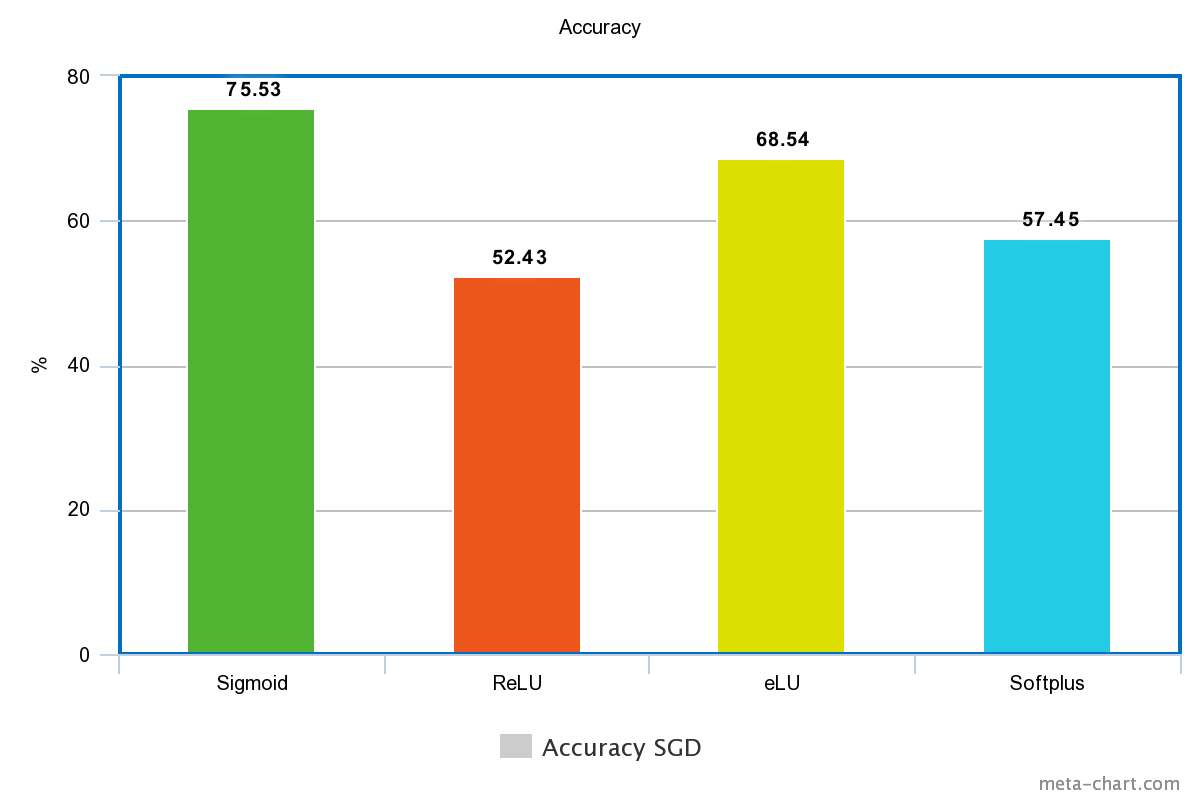
\includegraphics[width=13cm]{SGD_accuracy_tensorflow.png}
	\caption{ Accuracy of Stacked Autoencoder with Momentum optimizer for different activation, Unsupervised Learning }
	\label{fig:acc_sgd_tf}
	\end{figure}
	\clearpage
 
	\begin{table}[ht]
	\centering
	\captionsetup{justification=centering,margin=2cm}
	\begin{tabular}{|c|c|c|c|c|c|}
	\hline
	\textbf{Attack Types} & \textbf{Total Samples} & \textbf{Sigmoid} & \textbf{ReLu} & \textbf{eLu} & \textbf{Softplus} \\ \hline
	\textbf{Normal}       & 10003                  & 9696            & 9106         & 9792        & 8802           \\ \hline
	\textbf{DoS}          & 7164                  & 5392            & 2714         & 4524        & 3078             \\ \hline
	\textbf{Probe}        & 2421                  & 1937             & 0          & 1136         & 1071              \\ \hline
	\textbf{U2R}          & 2887                    & 0             & 0           & 0          & 0               \\ \hline
	\textbf{R2L}          & 67                     & 0               & 0            & 0           & 0                \\ \hline
	\end{tabular}
	\caption{Number of samples correctly identified for Momentum Optimizer with different Activation functions, Unsupervised Learning}
	\label{confusion_sgd_tf}
	\end{table}
  
  As we can see that with \textit{Adam Optimizer}, only the \textit{sigmoid activation} was able to classify correctly different attack types,\text{ ReLU, eLU, and Softpuls} were unable to classify single \textit{Probing, U2R and R2L} attacks.
%%%%%%%%%%%%%%%% sigmoid adam tf %%%%%%%%%%%%%%%%%%%%%%%%%%%%%%	
   
   \subsection{Sigmoid Activation}
 	 \begin{table}[ht]
		\centering
		\captionsetup{justification=centering,margin=2cm}
		\begin{tabular}{|c|c|c|c|}
		\hline
		\textbf{Attack Types} & \textbf{Precision} & \textbf{Recall} & \textbf{F1-score} \\ \hline
		\textbf{Normal}       & 0.6663             & 0.9693          & 0.7897            \\ \hline
		\textbf{DoS}          & 0.9608             & 0.7527          & 0.8441            \\ \hline
		\textbf{Probe}        & 0.8149             & 0.8001          & 0.8074            \\ \hline
		\textbf{U2R}          & 0.0000             & 0.0000          & 0.0000            \\ \hline
		\textbf{R2L}          & 0.0000             & 0.0000          & 0.0000            \\ \hline
		\end{tabular}
		\caption{Precision Recall and F1-Score Values of Sigmoid Activation for Momentum Optimizer, Unsupervised Learning}
		\label{classification sigmoid sgd tf}
		\end{table} 
  
  %%%%%%%%%%%%%% Relu adam tf%%%%%%%%%%%%%%%%%%%%%%%%%%%%%%%%%%%%%%%%%%%%%%%%%
  
  \subsection{ReLU Activation}
  \begin{table}[ht]
		\centering
		\captionsetup{justification=centering,margin=2cm}
		\begin{tabular}{|c|c|c|c|}
		\hline
		\textbf{Attack Types} & \textbf{Precision} & \textbf{Recall} & \textbf{F1-score} \\ \hline
		\textbf{Normal}       & 0.4904             & 0.9103          & 0.6374            \\ \hline
		\textbf{DoS}          & 0.6927             & 0.3788          & 0.4898            \\ \hline
		\textbf{Probe}        & 0.0000             & 0.0000          & 0.0000            \\ \hline
		\textbf{U2R}          & 0.0000             & 0.0000          & 0.0000            \\ \hline
		\textbf{R2L}          & 0.0000             & 0.0000          & 0.0000            \\ \hline
		\end{tabular}
		\caption{Precision Recall and F1-Score Values of ReLU Activation for Momentum Optimizer, Unsupervised Learning}
		\label{classification ReLU sgd tf}
		\end{table} 
\clearpage
 %%%%%%%%%%%%%% ELU adam tf %%%%%%%%%%%%%
   \subsection{eLU Activation}
  \begin{table}[h]
		\centering
		\captionsetup{justification=centering,margin=2cm}
		\begin{tabular}{|c|c|c|c|}
		\hline
		\textbf{Attack Types} & \textbf{Precision} & \textbf{Recall} & \textbf{F1-score} \\ \hline
		\textbf{Normal}       & 0.6059             & 0.9789          & 0.7485            \\ \hline
		\textbf{DoS}          & 0.9558             & 0.6315          & 0.7605            \\ \hline
		\textbf{Probe}        & 0.6940             & 0.4692          & 0.5599            \\ \hline
		\textbf{U2R}          & 0.0000             & 0.0000          & 0.0000            \\ \hline
		\textbf{R2L}          & 0.0000             & 0.0000          & 0.0000            \\ \hline
		\end{tabular}
		\caption{Precision Recall and F1-Score Values of eLU Activation for Momentum Optimizer, Unsupervised Learning}
		\label{classification eLU sgd tf}
		\end{table} 

   %%%%%%%%%%%%%% Softplus adam tf %%%%%%%%%%%%%
   \subsection{Softplus Activation}
  \begin{table}[h]
		\centering
		\captionsetup{justification=centering,margin=2cm}
		\begin{tabular}{|c|c|c|c|}
		\hline
		\textbf{Attack Types} & \textbf{Precision} & \textbf{Recall} & \textbf{F1-score} \\ \hline
		\textbf{Normal}       & 0.5827             & 0.8799          & 0.7011            \\ \hline
		\textbf{DoS}          & 0.9716             & 0.4296          & 0.5958            \\ \hline
		\textbf{Probe}        & 0.2909             & 0.4424          & 0.3510            \\ \hline
		\textbf{U2R}          & 0.0000             & 0.0000          & 0.0000            \\ \hline
		\textbf{R2L}          & 0.0000             & 0.0000          & 0.0000            \\ \hline
		\end{tabular}
		\caption{Precision Recall and F1-Score Values of Softplus Activation for Momentum Optimizer, Unsupervised Learning}
		\label{classification softplus mom tf}
		\end{table} 











  
\end{appendices}

\end{document}
